\NeedsTeXFormat{LaTeX2e}

\documentclass{jfp}

\usepackage{code}
%\usepackage{amsmath}
%\usepackage{times}
\usepackage{comment}
\usepackage{url}
\usepackage{fancyvrb}
\usepackage{graphics}
\usepackage{boxedminipage}

\usepackage[bookmarks=false,%
            colorlinks,linkcolor=black,urlcolor=blue,%
            pdfauthor={Oleg and Ralf},%
            pdftitle={OOHaskell}]{hyperref}

\DefineShortVerb{\|}
%\DefineVerbatimEnvironment{code}{Verbatim}{xleftmargin=\mathindent,commandchars=\\\{\},fontsize=\small}
% \setlength{\parskip}{0pt}
%\newlength{\mathindent}
%\setlength{\mathindent}{1em}


% Macros for notes to each other in the text
\newcommand{\keean}[1]{{\it [Keean says: #1]}}
\newcommand{\oleg}[1]{{\it [Oleg says: #1]}}
\newcommand{\ralf}[1]{{\it [Ralf says: #1]}}

\newcommand{\noskip}{\topsep0pt \parskip0pt \partopsep0pt}
\newcommand{\w}[1]{\textit{#1}}
\newcommand{\cmt}[1]{\mbox{\textrm{\emph{#1}}}}
\newcommand{\mysize}{\small}
\newcommand{\myskip}{\smallskip}
\newcommand{\antiskip}{\vspace{-25\in}}
\newcommand{\myinput}[1]{The content of this section is not yet released.}
\newcommand{\HList}{\textsc{HList}}
\newcommand{\undefined}{\ensuremath{\bot}}
\newcommand{\Forall}{\ensuremath{\forall}}
 

\begin{document}

%\conferenceinfo{WXYZ '05}{date, City.} 
%\copyrightyear{2005} 
%\copyrightdata{supplied by printer} 
 
%\title[Journal of Functional Programming]
\title{Haskell's overlooked object system\\
{\normalsize ---~DRAFT OF \today~---}}

\author[O. Kiselyov and R. L{\"a}mmel]{Oleg Kiselyov\\%FNMOC, Monterey, CA
Fleet Numerical Meteorology and Oceanography Center, Monterey, CA
\and
Ralf L{\"a}mmel\\Microsoft Corp., Redmond, WA}



\maketitle

\begin{abstract}

Haskell provides type-class-based bounded polymorphism as opposed to
subtype polymorphism of object-oriented languages such as Java and
OCaml. It is a contentious question whether Haskell (alone or with
extensions) can fully support conventional object-oriented programming
with encapsulation, mutable state, inheritance, overriding, statically
checked implicit and explicit subtyping, and so on.

We have constructively shown that Haskell \emph{as it is} supports all
the conventional OO features plus more advanced ones, including
first-class lexically scoped classes, implicitly polymorphic classes,
flexible multiple inheritance, and safe covariant arguments. 
We address the particular challenge
to preserve Haskell's type inference even for objects and
object-operating functions. Many of the features we get ``for free'':
the type system of Haskell turns out to be a great help and a guide
rather than a hindrance.

The OO features are introduced in Haskell as the OOHaskell
\emph{library}, non-trivially based on the \HList\ library of
extensible polymorphic records with first-class labels and
subtyping. The library sample code, which is patterned after the
examples found in OO textbooks and programming language tutorials,
including the OCaml object tutorial, demonstrates that OO code translates
into OOHaskell in an intuition-preserving way: essentially
expression-by-expression, without requiring global transformations.

OOHaskell lends itself as a sandbox for typed OO language design.

\medskip

\noindent
\textbf{Keywords:} Object-oriented functional programming, Class type
inference, Typed object-oriented language design, Heterogeneous
collections, ML-ART, Mutable objects

\end{abstract}



\makeatactive

\newpage 

{

%\small
\footnotesize

\setcounter{tocdepth}{3}
\tableofcontents

}

\newpage



%%%%%%%%%%%%%%%%%%%%%%%%%%%%%%%%%%%%%%%%%%%%%%%%%%%%%%%%%%%%%%%%%%%%%%%%%%%%%
%%%%%%%%%%%%%%%%%%%%%%%%%%%%%%%%%%%%%%%%%%%%%%%%%%%%%%%%%%%%%%%%%%%%%%%%%%%%%
%%%%%%%%%%%%%%%%%%%%%%%%%%%%%%%%%%%%%%%%%%%%%%%%%%%%%%%%%%%%%%%%%%%%%%%%%%%%%



\section{Introduction}

The topic of object-oriented programming in the functional language
Haskell is raised time and again on programming language mailing
lists, on programming tutorial websites, and in verbal communication
at programming language conferences with remarkable
intensity. Dedicated OO Haskell language extensions have been
proposed; specific OO idioms have been encoded in
Haskell~\cite{HS95,GJ96,FLMPJ99, SPJ01,Nordlander02,MonadReader3}.
The interest in this topic is not at all restricted to Haskell
researchers and practioners since there is a fundamental and unsettled
question~---~a question that is addressed in the present paper:\footnote{On a more anecdotal account, we have collected
informative pointers to mailing list discussions, which document the
unsettled understanding of OO programming in Haskell and the relation
between OO classes and Haskell's type classes: {\scriptsize
\url{http://www.cs.mu.oz.au/research/mercury/mailing-lists/mercury-users/mercury-users.0105/0051.html},
\url{http://www.talkaboutprogramming.com/group/comp.lang.functional/messages/47728.html},
\url{http://www.haskell.org/pipermail/haskell/2003-December/013238.html},
\url{http://www.haskell.org/pipermail/haskell-cafe/2004-June/006207.html},
\url{http://www.haskell.org//pipermail/haskell/2004-June/014164.html}}}

\begin{center}\itshape
What is the relation between type-class-bounded and subtype polymorphism?
\end{center}

\noindent
In this research context, we specifically (and emphatically) restrict
ourselves to the existing Haskell language (Haskell~98 and common
extensions where necessary), i.e., no new Haskell extensions are to be
proposed. As we will substantiate, this restriction is adequate, as it
allows us to deliver a meaningful and momentous answer to the
aforementioned question. At a more detailed level, we offer the
following motivation for research on OO programming in Haskell:
%
\begin{itemize}

\item
In an \emph{intellectual} sense, one may wonder whether Haskell's
advanced type system is expressive enough to model object types,
inheritance, subtyping, virtual methods, etc. No general, conclusive
result has been available so far.

\smallskip

\item
In a \emph{practical} sense, one may wonder whether we can faithfully
transport imperative OO designs from, say, C\#, C++, Eiffel, Java, VB
to Haskell~---~without totally rewriting the design and without
foreign-language interfacing?

\smallskip

\item From a \emph{language design} perspective, Haskell has a strong
record in prototyping semantics and encoding abstraction mechanisms,
but one may wonder whether Haskell can perhaps even serve as a sandbox
for design of typed object-oriented languages so that one can play
with new ideas without the immediate need to write or modify a
compiler.

\smallskip

\item In an \emph{educational} sense, one may wonder whether
more or less advanced functional and object-oriented programmers can
improve their understanding of Haskell's type system and OO concepts
by looking into the pros and cons of different OO encoding options in
Haskell.

\end{itemize}

\smallskip

This paper delivers substantiated, positive answers to these
questions. We describe OOHaskell~---~a Haskell-based library for (as
of today: imperative) OO programming in Haskell. OOHaskell delivers
Haskell's ``overlooked'' object system. The key to this result is a
good deal of exploitation of Haskell's advanced type system
\emph{combined} with a careful identification of a suitable object
encoding. We instantiate, combine and enhance existing encoding
techniques (such as~\cite{PT94,ML-ART,AC96}) to Haskell, while aiming
at a practical object system and while also blending well with the
host language~---~Haskell. We take advantage of our previous work on
heterogeneous collections~\cite{HLIST-HW04} (the \HList\ library).
More generallly, we put type-class-based programming for type-level
functionality to work~\cite{Hallgren01,Fake,NTGS02,NTGS01}.

\medskip

\noindent
The simplified story is the following:

\noindent
- Classes are represented as functions that are in fact object generators.

\noindent
- State is maintained through references allocated by object generators.

\noindent
- Objects are represented as records of closures with a component for each method.

\noindent
- Methods are monadic functions that thereby can access state.

\noindent
- We use \HList's polymorphic extensible records with structural subtyping.

\noindent
- We use type-class-based functionality to program the typed object system.

\medskip

\noindent
To deliver a faithful, convenient and comprehensive object system,
several techniques had to be discovered and combined. For instance,
extra effort was needed to preserve Haskell's type inference for OO
programming idioms (as opposed to explicit type declarations or type
constraints for classes, methods, and up-casts). The obtained result,
OOHaskell, delivers an amount of polymorphism and type inference that
is unprecedenced. Extra effort was also needed in order to deploy
value recursion for closing object generators. This approach is known
to require special care if it is meant to be safe.\footnote{Quoted
from~\cite{ML-ART}: ``Object encoding, based on record calculi, has
revealed severe difficulties, mainly due to over-reliance on recursive
values.'' We will show OOHaskell partially lifts these difficulties
through a combination of laziness and operator-suite design.} In order
to fully appreciate the object system of OOHaskell, we also review
less sophisticated, less favourable encoding alternatives.

Not only OOHaskell provides the conventional OO idioms; we have also
language-engineered several features that are either bleeding-edge or
unattainable in mainstream OO languages: for example, first-class
classes and class closures; statically type-checked collection classes
with bounded polymorphism of implicit collection arguments; multiple
inheritance with user-controlled sharing; safe covariant argument
subtyping. It is especially remarkable that these and more familiar
object-oriented features are not introduced by fiat~---~we get them
for free. For example, the type of a collection with bounded
polymorphism of elements is inferred automatically by the
compiler. Also, abstract classes are uninstantiatable not because we
say so but because the program will not typecheck otherwise. Co- and
contra-variant subtyping rules and the safety conditions for the
co-variant method argument types are checked automatically without any
programming on our part. These facts suggest that (OO)Haskell lends
itself as prime environment for typed object-oriented language design.



%%%%%%%%%%%%%%%%%%%%%%%%%%%%%%%%%%%%%%%%%%%%%%%%%%%%%%%%%%%%%%%%%%%%%%%%%%%%%
%%%%%%%%%%%%%%%%%%%%%%%%%%%%%%%%%%%%%%%%%%%%%%%%%%%%%%%%%%%%%%%%%%%%%%%%%%%%%
%%%%%%%%%%%%%%%%%%%%%%%%%%%%%%%%%%%%%%%%%%%%%%%%%%%%%%%%%%%%%%%%%%%%%%%%%%%%%

\newpage

\subsection*{Road-map of this paper}

\begin{itemize}
\item Sec.~\ref{S:shapes}: We encode a tutorial OO example both in C++ and OOHaskell.
\item Sec.~\ref{S:poor}: We review alternative object encodings in Haskell~98 and beyond.
\item Sec.~\ref{S:OOHaskell}: We describe OOHaskell's idioms for OO programming.
\item Sec.~\ref{S:discuss}: We assess OOHaskell complete with directions for future work.
\item Sec.~\ref{S:related}: We discuss related work.
\item Sec.~\ref{S:concl}: We conclude the paper.
\end{itemize}

\noindent
The main section, Sec.~\ref{S:OOHaskell}, is written in tutorial style,
as to ease digestion of all techniques, as to encourage OO programming
and OO language design experiments. There is an extended code
distribution available.\footnote{The source code can be downloaded at
\url{http://www.cwi.nl/~ralf/OOHaskell/}, and it is subject to 
a very liberal license (MIT/X11 style). As of writing, the actual code
commits to a few specific extensions of the GHC implementation of
Haskell~---~for reasons of convenience. In principle, Haskell~98 +
multi-parameter classes with functional dependencies is sufficient.}



%%%%%%%%%%%%%%%%%%%%%%%%%%%%%%%%%%%%%%%%%%%%%%%%%%%%%%%%%%%%%%%%%%%%%%%%%%%%%
%%%%%%%%%%%%%%%%%%%%%%%%%%%%%%%%%%%%%%%%%%%%%%%%%%%%%%%%%%%%%%%%%%%%%%%%%%%%%
%%%%%%%%%%%%%%%%%%%%%%%%%%%%%%%%%%%%%%%%%%%%%%%%%%%%%%%%%%%%%%%%%%%%%%%%%%%%%



\section{The folklore `shapes' example}
\label{S:shapes}

One of the main goals of this paper is to be able represent the
conventional OO code, in as straightforward way as possible.  The
implementation of our system may be not for the feeble at
heart~---~however, the user of the system must be able to write
conventional OO code without understanding the complexity of the
implementation. Throughout the paper, we illustrate OOHaskell with a
series of practical examples as they are commonly found in OO
textbooks and programming language tutorials. In this section, we
begin with the so-called `shapes' example.

We face a type for `shapes' and two subtypes for `rectangles' and
`circles'; see Fig.~\ref{F:shapes}. Shapes maintain coordinates as
state. Shapes can be moved around and drawn. The exercise shall be to
place objects of \emph{different} kinds of shapes in a collection and
to iterate over them as to draw the shapes. It turns out that this
example is a crisp OO benchmark.\footnote{The `shapes' problem
has been designed by Jim Weirich and deeply explored by him and Chris
Rathman. See the multi-lingual collection `OO Example Code' by Jim
Weirich at \url{http://onestepback.org/articles/poly/}; see also an
even heavier collection `OO Shape Examples' by Chris Rathman at
\url{http://www.angelfire.com/tx4/cus/shapes/}.}



%%%%%%%%%%%%%%%%%%%%%%%%%%%%%%%%%%%%%%%%%%%%%%%%%%%%%%%%%%%%%%%%%%%%%%%%%%%%%
%%%%%%%%%%%%%%%%%%%%%%%%%%%%%%%%%%%%%%%%%%%%%%%%%%%%%%%%%%%%%%%%%%%%%%%%%%%%%
%%%%%%%%%%%%%%%%%%%%%%%%%%%%%%%%%%%%%%%%%%%%%%%%%%%%%%%%%%%%%%%%%%%%%%%%%%%%%



\begin{figure}[t!]
\bigskip
\begin{center}
\resizebox{.73\textwidth}{!}{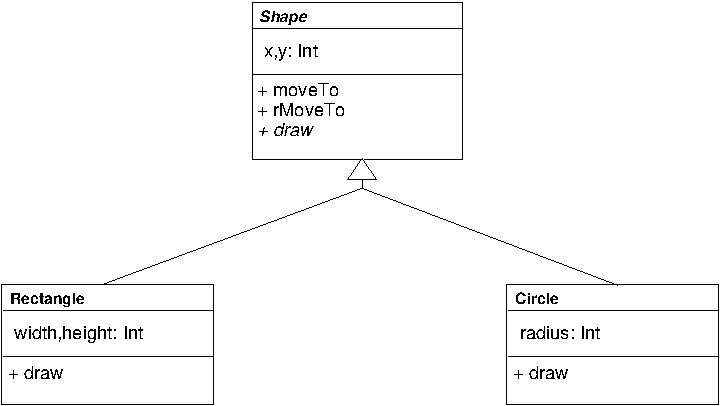
\includegraphics{shapes.pdf}}
\end{center}
\caption{Shapes with state and a subtype-specific draw method}
\label{F:shapes}
\bigskip
\end{figure}



%%%%%%%%%%%%%%%%%%%%%%%%%%%%%%%%%%%%%%%%%%%%%%%%%%%%%%%%%%%%%%%%%%%%%%%%%%%%%
%%%%%%%%%%%%%%%%%%%%%%%%%%%%%%%%%%%%%%%%%%%%%%%%%%%%%%%%%%%%%%%%%%%%%%%%%%%%%
%%%%%%%%%%%%%%%%%%%%%%%%%%%%%%%%%%%%%%%%%%%%%%%%%%%%%%%%%%%%%%%%%%%%%%%%%%%%%



\subsection{C++ reference encoding}

The type of shapes can be defined as a C++ class as follows:

\begin{Verbatim}[fontsize=\small,commandchars=\|\!\@]
 class Shape {
 public:
\end{Verbatim}

\begin{Verbatim}[fontsize=\small,commandchars=\|\!\@]
   // |cmt!Constructor method@
   Shape(int newx, int newy) {
     x = newx;
     y = newy;
   }
\end{Verbatim}

\begin{Verbatim}[fontsize=\small,commandchars=\|\!\@]
   // |cmt!Accessors@
   int getX() { return x; }
   int getY() { return y; }
   void setX(int newx) { x = newx; }
   void setY(int newy) { y = newy; }
\end{Verbatim}

\begin{Verbatim}[fontsize=\small,commandchars=\|\!\@]
   // |cmt!Move shape position@
   void moveTo(int newx, int newy) {
      setX(newx);
      setY(newy);
   }
\end{Verbatim}

\begin{Verbatim}[fontsize=\small,commandchars=\|\!\@]
   // |cmt!Move shape relatively@
   void rMoveTo(int deltax, int deltay) {
      moveTo(getX() + deltax, getY() + deltay);
   }
\end{Verbatim}

\begin{Verbatim}[fontsize=\small,commandchars=\|\!\@]
   // |cmt!An abstract draw method@
   virtual void draw() = 0;
\end{Verbatim}

\begin{Verbatim}[fontsize=\small,commandchars=\|\!\@]
 // |cmt!Private data@
 private:
   int x;
   int y;
 }
\end{Verbatim}

The @x@, @y@ coordinates are private, but they can be accessed through
getters and setters. The methods for access and moving shapes are
inherited to the subclasses of @Shape@. The @draw@ method is virtual
and even abstract; hence concrete subclasses must implement @draw@.

\newpage 

The subclass @Rectangle@ is derived as follows:

\begin{Verbatim}[fontsize=\small,commandchars=\|\!\@]
 class Rectangle: public Shape {
 public:
\end{Verbatim}

\begin{Verbatim}[fontsize=\small,commandchars=\|\!\@]
   // |cmt!Constructor method@
   Rectangle(int newx, int newy, int newwidth, int newheight)
            : Shape(newx, newy) {
     setWidth(newwidth);
     setHeight(newheight);
   }
\end{Verbatim}

\begin{Verbatim}[fontsize=\small,commandchars=\|\!\@]
   // |cmt!Accessors@
   int getWidth()  { return width; }
   int getHeight() { return height; }
   void setWidth(int newwidth)   { width = newwidth; }
   void setHeight(int newheight) { height = newheight; }
\end{Verbatim}

\begin{Verbatim}[fontsize=\small,commandchars=\|\!\@]
   // |cmt!Implementation of the abstract draw method@
   void draw() {
     cout << "Drawing a Rectangle at:("
          << getX() << "," << getY()
          << "), width " << getWidth()
          << ", height " << getHeight() << endl;
   }
\end{Verbatim}

\begin{Verbatim}[fontsize=\small,commandchars=\|\!\@]
 // |cmt!Additional private data@
 private:
    int width;
    int height;
 };
\end{Verbatim}

For brevity, we elide the similar derivation of the subclass @Circle@:

\begin{code}
 class Circle : public Shape {
  Circle(int newx, int newy, int newradius)
        : Shape(newx, newy) { ... }
  ...
 }
\end{code}

The following code block exercices the construction of different shape
objects and the invocation of their methods. More precisely, we place
two shapes of different kinds in an array, @scribble@, and we then
perform a loop over the array such that the shape objects are drawn:

\begin{code}
 Shape *scribble[2];
 scribble[0] = new Rectangle(10, 20, 5, 6);
 scribble[1] = new Circle(15, 25, 8);
 for (int i = 0; i < 2; i++) {
   scribble[i]->draw();
   scribble[i]->rMoveTo(100, 100);
   scribble[i]->draw();
 }
\end{code}

We note that the loop over @scribble@ exercises subtyping
polymorphism; the actually executed implementation of the @draw@
method differs per element in the array. The program run produces the
following output~---~due to the logging-like implementations of the
@draw@ method:

\begin{code}
 Drawing a Rectangle at:(10,20), width 5, height 6
 Drawing a Rectangle at:(110,120), width 5, height 6
 Drawing a Circle at:(15,25), radius 8
 Drawing a Circle at:(115,125), radius 8
\end{code}



%%%%%%%%%%%%%%%%%%%%%%%%%%%%%%%%%%%%%%%%%%%%%%%%%%%%%%%%%%%%%%%%%%%%%%%%%%%%%
%%%%%%%%%%%%%%%%%%%%%%%%%%%%%%%%%%%%%%%%%%%%%%%%%%%%%%%%%%%%%%%%%%%%%%%%%%%%%
%%%%%%%%%%%%%%%%%%%%%%%%%%%%%%%%%%%%%%%%%%%%%%%%%%%%%%%%%%%%%%%%%%%%%%%%%%%%%



\subsection{OOHaskell encoding}

We will now show an OOHaskell encoding, which happens to pleasantly
mimic the C++ encoding, while any remaining deviations are
appreciated. Most notably, we are going to leverage type inference.
We are not going to define \emph{any} type~---~nevertheless the code
will be fully statically typed, of course.

\smallskip

Here is the OOHaskell rendering of the shape class:

\begin{Verbatim}[fontsize=\small,commandchars=\|\{\}]
 -- |cmt{Object generator for shapes}
 shape newx newy self
   = do
	-- |cmt{Create references for private state}
        x <- newIORef newx
        y <- newIORef newy
\end{Verbatim}

\begin{Verbatim}[fontsize=\small,commandchars=\|\{\}]
	-- |cmt{Return object as record of methods}
        returnIO $  getX     .=. readIORef x
                .*. getY     .=. readIORef y
                .*. setX     .=. (\newx -> writeIORef x newx)
                .*. setY     .=. (\newy -> writeIORef y newy)
                .*. rMoveTo  .=. (\deltax deltay -> 
\end{Verbatim}

\begin{Verbatim}[fontsize=\small,commandchars=\|\{\}]
                            do
                              x <- self # getX
                              y <- self # getY
                              (self # setX) (x + deltax)
                              (self # setY) (y + deltay) )
         .*. emptyRecord
\end{Verbatim}

%% $

Classes become \emph{functions that take constructor arguments plus a
self reference and that return a computation whose result is the new
object~---~a record of methods}. We can invoke methods of the same
object through @self@; cf.\ the method invocation @self@~@#@~@getX@
and others. (We use the infix operator @#@ to denote method
invocation.) We use mutable objects, implemented via @IORef@
(@STRef@ also suffice). Since most OO systems in practical use
have mutable state, OOHaskell does not yet offer
\emph{functional objects}, which are known to be challenging on their
own. We defer functional objects to a topic for future work. 

We use the extensible records of the \HList\ library~\cite{HLIST-HW04},
hence:
%
\begin{itemize}\noskip
\item @emptyRecord@ denotes what the name promises.
\item @(.*.)@ denotes (right-associative) record extension.
\item @(.=.)@ denotes record-component construction: \w{label} @.=.@ \w{value}.
\item Labels are defined according to a trivial scheme, which we will explain later.
\end{itemize}
%
(We note that the abstract @draw@ method is not mentioned in the
OOHaskell code because it is not used in any other method, neither did
we dare declaring its type. As a side effect, the object generator
@shape@ is instantiable whereas the explicit declaration of the
abstract @draw@ method made the C++ class @Shape@ uninstantiable. We
will later show how to add similar declarations in OOHaskell.)

\medskip

\noindent
We continue with the OOHaskell code for the shapes example.

\begin{Verbatim}[fontsize=\small,commandchars=\|\{\}]
 -- |cmt{Object generator for rectangles}
 rectangle x y width height self
   = do
        -- |cmt{Invoke object generator of superclass}
        super <- shape x y self
\end{Verbatim}

\begin{Verbatim}[fontsize=\small,commandchars=\|\{\}]
        -- |cmt{Create references for extended state}
        w <- newIORef width
        h <- newIORef height
\end{Verbatim}

\begin{Verbatim}[fontsize=\small,commandchars=\|\{\}]
	-- |cmt{Return object as record of methods}
        returnIO $
\end{Verbatim}

%% $

\begin{Verbatim}[fontsize=\small,commandchars=\|\{\}]
            // |cmt{Accessors}
            getWidth  .=. readIORef w
        .*. getHeight .=. readIORef h
        .*. setWidth  .=. (\neww -> writeIORef w neww)
        .*. setHeight .=. (\newh -> writeIORef h newh)
\end{Verbatim}

\begin{Verbatim}[fontsize=\small,commandchars=\|\{\}]
            // |cmt{Implementation of the abstract draw method}
        .*. draw .=. 
             do
                putStr  "Drawing a Rectangle at:(" <<
                        self # getX << ls "," << self # getY <<
                        ls "), width " << self # getWidth <<
                        ls ", height " << self # getHeight << ls "\n"
\end{Verbatim}

\begin{Verbatim}[fontsize=\small,commandchars=\|\{\}]
            // |cmt{Rectangle records start from shape records}
        .*. super
\end{Verbatim}

This snippet illustrates the essence of inheritance in OOHaskell.
Object generation for the supertype is made part of the monadic
sequence that defines object generation for the subtype; @self@ is
passed from the subtype to the supertype. Subtype records are derived
from supertype records through record extension (or potentially also
record updates).

As in the C++ case, we elide the derivation of the object generators
for circles:

\begin{code}
 circle newx newy newradius self
  = do
       super <- shape newx newy self
       ...
       returnIO ... .*. super
\end{code}

\newpage

Ultimately, here is the OOHaskell rendering of the `scribble loop':

\begin{Verbatim}[fontsize=\small,commandchars=\|\{\}]
 -- |cmt{Object construction and invocation as a monadic sequence}
 myOOP = do
\end{Verbatim}

\begin{Verbatim}[fontsize=\small,commandchars=\|\{\}]
          -- |cmt{Construct objects}
          s1 <- mfix (rectangle (10::Int) (20::Int) 5 6)
          s2 <- mfix (circle (15::Int) 25 8)
\end{Verbatim}

\begin{Verbatim}[fontsize=\small,commandchars=\|\{\}]
          -- |cmt{Create a list of different shapes}
          let scribble = consLub s1 (consLub s2 nilLub)
\end{Verbatim}

\begin{Verbatim}[fontsize=\small,commandchars=\|\{\}]
          -- |cmt{Loop over list with normal monadic map}
          mapM_ (\shape -> do
                            shape # draw
                            (shape # rMoveTo) 100 100
                            shape # draw)
                scribble
\end{Verbatim}

The use of @mfix@ (an analogue of @new@) reflects that object
generators take `self' and construct (part of) it. Open recursion
enables inheritance. Let us look at the @let scribble@ \ldots binding.
We cannot \emph{directly} place rectangles and circles in a normal
Haskell list~---~the following let binding cannot possibly type check:

\begin{Verbatim}[fontsize=\small,commandchars=\|\{\}]
          let scribble = [s1,s2] -- s1 and s2 are of different types!
\end{Verbatim}

\noindent
So instead we need to homogenise the types of @s1@ and @s2@ while
forming a Haskell list. To this end, we use special list constructors
@nilLub@ and @consLub@ as opposed to the normal list constructors @[]@
and @(:)@. These new constructors coerce the list elements to the
least-upper bound type of all the element types. Incidentally, if the
`intersection' of the type of the objects @s1@ and @s2@ does not
include the used methods @draw@ and @rMoveTo@, we get a static type
error which literally says so. As a result, the original for-loop can
be carried out in the native Haskell way: a normal (monadic) list map
over a normal Haskell list of shapes. Hence, we have exercised a
faithful model of subtype polymorphism, which also allows for (almost)
implicit subtyping. OOHaskell provides several subtyping models, as we
will study later.



%%%%%%%%%%%%%%%%%%%%%%%%%%%%%%%%%%%%%%%%%%%%%%%%%%%%%%%%%%%%%%%%%%%%%%%%%%%%%
%%%%%%%%%%%%%%%%%%%%%%%%%%%%%%%%%%%%%%%%%%%%%%%%%%%%%%%%%%%%%%%%%%%%%%%%%%%%%
%%%%%%%%%%%%%%%%%%%%%%%%%%%%%%%%%%%%%%%%%%%%%%%%%%%%%%%%%%%%%%%%%%%%%%%%%%%%%



\subsection{Discussion of the example}

\subsubsection{Classes vs.\ interfaces}

The C++ code should not be misunderstood to suggest that \emph{class}
inheritance is the only OO design option for the shapes hierarchy. In
a Java-like language, one may want to model @Shape@ as an
\emph{interface}, say, @IShape@, with @Rectangle@ and @Circle@ as classes
implementing this interface. This design would not allow us to reuse
the implementations of the accessors and the move methods. So one may
want to combine interface polymorphism \emph{and} class
inheritance. That is, the classes @Rectangle@ and @Circle@ will be
rooted by an additional implementation class for shapes, say @Shape@,
which hosts implementations shared among different shape
classes~---~incidentally a part of the @IShape@ interface. The
remainder of the @IShape@ interface, namely the @draw@ method in our
example, is implemented in @Rectangle@ and @Circle@.

More generally, OO designs that employ interface polymorphism alone
are rare, so we need to provide encodings for both OO interface
polymorphism \emph{and} OO class inheritance in OOHaskell. One may say
that the former mechanism is essentially covered by Haskell's type
classes (modulo the fact that we would still need an object
encoding). The latter mechanism is specifically covered by original
HList and OOHaskell contributions: structural subtyping polymorphism
for object types, based on extensible records and programmable
subtyping constraints. (We will discuss the use of \emph{nominal}
object types in OOHaskell as well.)



%%%%%%%%%%%%%%%%%%%%%%%%%%%%%%%%%%%%%%%%%%%%%%%%%%%%%%%%%%%%%%%%%%%%%%%%%%%%%
%%%%%%%%%%%%%%%%%%%%%%%%%%%%%%%%%%%%%%%%%%%%%%%%%%%%%%%%%%%%%%%%%%%%%%%%%%%%%
%%%%%%%%%%%%%%%%%%%%%%%%%%%%%%%%%%%%%%%%%%%%%%%%%%%%%%%%%%%%%%%%%%%%%%%%%%%%%



\subsubsection{The extensibility premise}
\label{S:ext}

The shapes example exercises the extensibility premise of the OO
paradigm. At the least, one may want to add new kinds of shapes
without rewriting existing code. A stronger (but quite common OO-like)
view on extensibity is that not even recompilation of existing code is
necessary. The basic OO paradigm has been critized~\cite{ZO04} in the
sense that it would emphasize extensibility in the subtyping
dimension, but it would neglect other dimensions such as the
functionality dimension~---~adding new functions on a preexising
subtyping hierarchy. While we agree with this overall criticism, we
restrict ourselves (in this paper) to the the established OO paradigm;
to the blend of OO and Haskell. (Incidentally, some of the
non-encapsulation-based encodings in Sec.~\ref{S:poor} show that
Haskell supports extensibility in both the data and the functionality
dimension.)



%%%%%%%%%%%%%%%%%%%%%%%%%%%%%%%%%%%%%%%%%%%%%%%%%%%%%%%%%%%%%%%%%%%%%%%%%%%%%
%%%%%%%%%%%%%%%%%%%%%%%%%%%%%%%%%%%%%%%%%%%%%%%%%%%%%%%%%%%%%%%%%%%%%%%%%%%%%
%%%%%%%%%%%%%%%%%%%%%%%%%%%%%%%%%%%%%%%%%%%%%%%%%%%%%%%%%%%%%%%%%%%%%%%%%%%%%



\subsubsection{The encapsulation premise}

Both the C++ encoding and the OOHaskell encoding of the shapes example
are faithful to the encapsulation premise of the OO paradigm. Again,
OO-like encapsulation is the subject of an unsettled debate in the
programming language community; in particular it is debated whether
such encapsulation is adequate for a functional style of programming.
We do not want to argue in any way; we simply want OOHaskell to
provide an object encoding that is compatible with the established OO
paradigm.



%%%%%%%%%%%%%%%%%%%%%%%%%%%%%%%%%%%%%%%%%%%%%%%%%%%%%%%%%%%%%%%%%%%%%%%%%%%%%
%%%%%%%%%%%%%%%%%%%%%%%%%%%%%%%%%%%%%%%%%%%%%%%%%%%%%%%%%%%%%%%%%%%%%%%%%%%%%
%%%%%%%%%%%%%%%%%%%%%%%%%%%%%%%%%%%%%%%%%%%%%%%%%%%%%%%%%%%%%%%%%%%%%%%%%%%%%



\subsubsection{Subtyping technicalities}

The ``scribble loop'' is by no means a contrived scenario. It is a
faithful instance of the ubiquitous composite design
pattern~\cite{GHJV94}. In terms of expressiveness and typing
challenges, this sort of loop on an array with shapes of different
kinds forces us to explore the tension between implicit and explicit
subtyping. As we will discuss, it is relatively straightforward to use
type-class-bounded polymorphism to represent subtype constraints. It
is however less straightforward to accumulate entities of different
subtypes in the same collection. With explicit subtyping (e.g., by
wrapping in a properly constrained existential envelope) the burden
would be on the side of the programmer. A key challenge for OOHaskell
was to make subtyping (almost) implicit in all the cases, where a OO
programmer would expect it. This is a particular area in which
OOHaskell goes beyond OCaml~\cite{OCaml}---~the de-facto leading
strongly typed functional object-oriented language. OOHaskell provides
a range of subtyping notions, including one that even allows for safe
downcasts for object types. This is again something that has not been
achieved in OCaml to date.



%%%%%%%%%%%%%%%%%%%%%%%%%%%%%%%%%%%%%%%%%%%%%%%%%%%%%%%%%%%%%%%%%%%%%%%%%%%%%
%%%%%%%%%%%%%%%%%%%%%%%%%%%%%%%%%%%%%%%%%%%%%%%%%%%%%%%%%%%%%%%%%%%%%%%%%%%%%
%%%%%%%%%%%%%%%%%%%%%%%%%%%%%%%%%%%%%%%%%%%%%%%%%%%%%%%%%%%%%%%%%%%%%%%%%%%%%



\section{Alternative Haskell encodings}
\label{S:poor}

OOHaskell goes particularly far in providing an object system, when
compared to conservative Haskell programming knowledge. In particular,
we put type-class-based programming to work. In this section, we will
discuss more conservative object encodings. We will review the
characteristics and limitations of the encodings. All of them require
boilerplate code from the programmer.

Some of the `conservative' encodings to come are nevertheless involved
and enlightening. Also, the full spectrum of encodings has not been
documented before~---~certainly not in a Haskell context. So we reckon
that their detailed analysis makes a useful contribution. Also,
several of the discussed techniques are actually used in OOHaskll,
while some of them are simply generalized through type-class-based
programming.

For most of this section, we will limit ourselves to Haskell~98. (By
constrast, OOHaskell requires several common Haskell~98 extensions.) 
Towards the end of the section, we will also investigate the value of
dismissing this restriction.



\subsection{Map subtype hierarchy to an algebraic datatype}
\label{S:lennart}

We begin with a trivial and concise encoding. The distinguishing
characteristic of this encoding is extreme simplicity.\footnote{Thanks
to Lennart Augustsson for pointing out this line of encoding.\\
Cf.\
\url{http://www.haskell.org/pipermail/haskell/2005-June/016061.html}}
In fact, we only use very basic Haskell~98 idioms. We should note that
the encoding is seriously limited in so far that it lacks
extensibility with regard to new forms of shapes (cf.\ Sec.~\ref{S:ext}).

We define an algebraic datatype for shapes, where each kind of shape
amounts to a constructor declaration. For readibility, we use labelled
fields instead of unlabelled constructor components.

\begin{code}
 data Shape =
              Rectangle { getX      :: Int
                        , getY      :: Int 
                        , getWidth  :: Int 
                        , getHeight :: Int }
            |
              Circle { getX      :: Int
                     , getY      :: Int 
                     , getRadius :: Int }
\end{code}

Both constructor declarations involve labelled fields for the $(x,y)$
position of a shape. While this reuseability dimension is not
emphasised at the datatype level, we can easily define reusable
setters for the position.  (There are some issues regarding type
safety, which we will address later.) For instance:

\begin{code}
 setX :: Int -> Shape -> Shape
 setX i s = s { getX = i } 
\end{code}

We can also define setters for @Rectangle@- and @Circle@-specific
fields. For instance:

\begin{code}
 setWidth :: Int -> Shape -> Shape
 setWidth i s = s { getWidth = i } 
\end{code}

It is also straightforward to define functions for moving around shapes:

\begin{code}
 moveTo :: Int -> Int -> Shape -> Shape
 moveTo x y = setY y . setX x 
\end{code}

\begin{code}
 rMoveTo :: Int -> Int -> Shape -> Shape
 rMoveTo deltax deltay s = moveTo x y s
  where
   x = getX s + deltax
   y = getY s + deltay
\end{code}

The function for drawing shapes properly discriminates on the kind of
shapes. That is, there is one equation per kind of shape. Subtype polymorphism
reduces to pattern matching, so to say:

\begin{code}
 draw :: Shape -> IO ()
\end{code}

\begin{code}
 draw s@(Rectangle _ _ _ _)
          =  putStrLn ("Drawing a Rectangle at:("
          ++ (show (getX s))
          ++ ","
          ++ (show (getY s))
          ++ "), width " ++ (show (getWidth s))
          ++ ", height " ++ (show (getHeight s)))
\end{code}

\begin{code}
 draw s@(Circle _ _ _)
          =  putStrLn ("Drawing a Circle at:("
          ++ (show (getX s))
          ++ ","
          ++ (show (getY s))
          ++ "), radius "
          ++ (show (getRadius s)))
\end{code}

It is now also trivial to build a collection of shapes of different
kinds and to iterate over it such that all shape entities are drawn.
This problem boils down to normal list processing in Haskell:

\begin{code}
 main =
       do
          let scribble = [ Rectangle 10 20 5 6
                         , Circle 15 25 8
                         ]
          mapM_ ( \x -> 
                    do
                       draw x
                       draw (rMoveTo 100 100 x))
                scribble
\end{code}



\paragraph{Assessment of the encoding}

\mbox{}

\begin{itemize}

\item
The encoding ignores the encapsulation premise of the OO paradigm.

\smallskip

\item
The foremost weakness of the encoding is the lack of extensibility.
The addition of a new kind of shape would require re-compilation of
all code; it would also require amendments of existing definitions or
declarations: the datatype declaration @Shape@ and the function
definition @draw@.

\smallskip

\item
A related weakness is that the overall scheme does not suggest a way
of dealing with virtual methods: introduce the type of a method for a
base type potentially with an implementation; define or override the
method for a subtype. We would need a scheme or an idiom that offers
(explicit and implicit) open recursion for datatypes and functions
defined on them.

\smallskip

\item
The setters @setX@ and @setY@ \emph{happen} to be total because all
constructors end up defining labelled fields @getX@ and @getY@. The
type system does \emph{not} prevent us from forgetting those labels
for some constructor. It is relatively easy to resolve this issue to
the slight disadvantage of conciseness. (For instance, we may
avoid labelling entirely, and use pattern matching instead. We may
also compose together rectangles and circles from common shape data
and deltas.)

\smallskip

\item
The use of a single algebraic datatype @Shape@ implies that
@Rectangle@- and @Circle@-specific functions cannot be defined as
total functions. Such biased functions, e.g., @setWidth@, are only
defined for certain constructors. It is possible to increase type
safety by making type disctinctions for different kinds of shapes, but
then we encounter the challenge of subtype polymorphism. This leads
us clearly out of the simpleminded encoding model at hand.

\end{itemize}



%%%%%%%%%%%%%%%%%%%%%%%%%%%%%%%%%%%%%%%%%%%%%%%%%%%%%%%%%%%%%%%%%%%%%%%%%%%%%
%%%%%%%%%%%%%%%%%%%%%%%%%%%%%%%%%%%%%%%%%%%%%%%%%%%%%%%%%%%%%%%%%%%%%%%%%%%%%
%%%%%%%%%%%%%%%%%%%%%%%%%%%%%%%%%%%%%%%%%%%%%%%%%%%%%%%%%%%%%%%%%%%%%%%%%%%%%



\subsection{Map object data to tail-polymorphic record types}
\label{S:burton}

There is a folklore technique for encoding extensible
records~\cite{Burton90} that we can use to model the shapes hierarchy
in Haskell~98. Combined with a simple usage pattern for type classes,
we can define reusable functionality and type-specific functionality
in a straightforward manner. The remaining challenge is then to enable
subtype-polymorphic collections. We address this challenge by making
different subtypes homogeneous through embedding shape subtypes into a
disjoint sum (Haskell's @Either@).

We begin with a datatype for extensible shapes; cf.\ @shapeTail@:

\begin{code}
 data Shape w =
      Shape { getX :: Int
            , getY :: Int
            , shapeTail :: w }
\end{code}

For convenience, we also provide a constructor for shapes:

\begin{code}
 shape x y w = Shape { getX = x
                     , getY = y
                     , shapeTail = w }
\end{code}

We can define setters and movers once and for all for all possible
extensions of @Shape@ by simply \emph{leaving the extension type
parametric}. The actual equations are literally the same as in the
previous section; so we only show the (different) parametrically
polymorphic types:

\begin{code}
 setX :: Int -> Shape w -> Shape w
 setY :: Int -> Shape w -> Shape w
 moveTo :: Int -> Int -> Shape w -> Shape w
 rMoveTo :: Int -> Int -> Shape w -> Shape w
\end{code}

(The polymorphism in an extension type @w@ expresses that the earlier
definitions on @Shape@ \ldots can clearly be instantiated to all
subtypes of @Shape@.) The @draw@ function must be placed in a
dedicated type class, @Draw@, because we anticipate the need to
provide type-specific implementations of @draw@. (One may compare this
style with C++ where one explicitly declares a method to be
(\emph{pure}) \emph{virtual}.)

\begin{code}
 class Draw w
  where
   draw :: Shape w -> IO ()
\end{code}

The derivation of extensions for rectangles and circles commences
according to a common scheme. We only show the details for rectangles.
We begin with the definition of the ``data delta'' contributed by
rectangles. We note that each such delta is again polymorphic in its
tail.

\begin{code}
 data RectangleDelta w =
      RectangleDelta { getWidth      :: Int 
                     , getHeight     :: Int
                     , rectangleTail :: w }
\end{code}

We can define the type of rectangles as an instance of @Shape@:

\begin{code}
 type Rectangle w = Shape (RectangleDelta w)
\end{code}

For convenience, we provide a constructor for rectangles. Here we fix
the tail of the rectangle delta to @()@. (We could still further
instantiate @Rectangle@ and define new constructors later, if
necessary.)

\begin{code}
 rectangle x y w h
  = shape x y $ RectangleDelta {
                  getWidth      = w
                , getHeight     = h
                , rectangleTail = () }
\end{code}

%% $

The definition of rectangle-specific setters involves nested record
manipulation:

\begin{code}
 setHeight :: Int -> Rectangle w -> Rectangle w
 setHeight i s = s { shapeTail = (shapeTail s) { getHeight = i } }
\end{code}

\begin{code}
 setWidth :: Int -> Rectangle w -> Rectangle w
 setWidth i s = s { shapeTail = (shapeTail s) { getWidth = i } }
\end{code}

The rectangle-specific @draw@ function is defined through a @Draw@ instance:

\begin{code}
 instance Draw (RectangleDelta w)
  where
   draw s
     =   putStrLn ("Drawing a Rectangle at:("
     ++ (show (getX s))
     ++ ","
     ++ (show (getY s))
     ++ "), width "
     ++ (show (getWidth (shapeTail s)))
     ++ ", height "
     ++ (show (getHeight (shapeTail s))))
\end{code}

The difficult part is the `scribble loop'. We cannot easily form a
collection of shapes of different kinds. For instance, the following
attempt will not type-check:

\begin{code}
 -- Wrong! There is no homogeneous element type.
 let scribble = [ rectangle 10 20 5 6
                , circle 15 25 8
                ]
\end{code}

There is a relatively simple technique to make rectangles and circles
homogeneous within the scope of the @scribble@ list and its clients.
We have to establish a sum type for the differnt kinds of
shapes.\footnote{Haskell~98 defines sums in the prelude: with the type
name @Either@, and the two constructors @Left@ and @Right@ for the
branches of the sum.} Using an appropriate helper, @tagShape@, for
embedding shapes into a sum type (Haskell's @Either@), we may
construct a homogeneous collection as follows:

\begin{code}
 let scribble = [ tagShape Left  (rectangle 10 20 5 6)
                , tagShape Right (circle 15 25 8)
                ]
\end{code}

The boilerplate operation for embedding is trivially defined as follows.

\begin{code}
 tagShape :: (w -> w') -> Shape w -> Shape w'
 tagShape f s = s { shapeTail = f (shapeTail s) }
\end{code}

Embedding (or tagging) does clearly not disturb the reusable
definitions of functions on @Shape w@. However, the loop over
@scribble@ refers to the @draw@ operation, which is defined for
@RectangleDelta@ and @CircleDelta@, but not for the sum over these two
types. we have to provide a trivial definition for @draw@, which will
actually suffice for arbitrarily nested sums over subtypes of @Shape@:

\begin{code}
 instance (Draw a, Draw b) => Draw (Either a b)
  where
   draw = eitherShape draw draw
\end{code}

Here, @eitherShape@ is variation on the normal fold operation for
sums, i.e., @either@. We discriminate on the @Left@ vs.\ @Right@ cases
for the tail of a shape datum. This boilerplate operation is
independent of @draw@, but specific to @Shape@.

\begin{code}
 eitherShape :: (Shape w -> t) -> (Shape w' -> t) -> Shape (Either w w') -> t
 eitherShape f g s
   = case shapeTail s of
       (Left s')  -> f (s { shapeTail = s' })
       (Right s') -> g (s { shapeTail = s' })
\end{code}



\paragraph{Assessment of the encoding}

\mbox{}

\begin{itemize}

\item
Again, the encoding ignores the encapsulation premise of the OO paradigm.

\smallskip

\item
The encoding does not have the basic extensibility problem of the
previous section. That is, we can introduce new kinds of shapes
without rewriting code, without recompiling type-specific code.

\smallskip

\item
Code that exercises subtype polymorphism may require revision. For
instance all program points that access a subtype-polymorphic
collection must agree on the formation of the sum type over specific
subtypes. If a new subtype must be covered, then the scattered
applications of embedding operations must be revised.

\smallskip

\item 
We fail to put Haskell's type inference to work as far as object types
are concerned. That is, we end up defining explicit datatypes for all
encoded classes. This is acceptable from a mainstream OO point of view
since nominal types (i.e., explicit types) dominate the OO
paradigm. However, in Haskell, we would like to do better by allowing
for inference of structural class and interface types. All subsequent
encodings of this section will share this problem. (By contrast,
OOHaskell provides full structural type inference.)

\smallskip

\item
It is annoying enough that the formation of a subtype-polymorphic
collection requires explicit tagging of all elements; cf.\ @Left@ and
@Right@. Worse than that is that the tagging is done on the delta
position of @Shape@. This makes this scheme non-compositional. (That
is, for each new base class, we would need to define functions like
@tagShape@ and @eitherShape@.) Also, it is nuisance that we need to
provide extra instances to operate on the sum type.

\smallskip

\item
The encoding of final methods and virtual methods differs essentially.
The former methods are encoded as parametric polymorphic functions
parameterized in the extension type. The latter methods are encoded as
type-class-bounded polymophic functions overloaded in the extension
type. An evolution of the final vs.\ virtual status would trigger code
rewriting.  One may suggest to use the scheme for virtuals generally
(combined with default methods so that implementations can be
reused). This may increase the amount of boilerplate code such as the
instances for @Either@.

\smallskip

\item
The subtyping hierarchy leaks into the encoding of subtype-speccific
accessors; cf.\ @setWidth@. The derivation chain from a base type
shows up as nesting depth in the record access pattern. One may factor
out these code patterns into accessor helpers per chain and overload
them so that all accessor can be coded in a uniform way. This would
also complicate the encoding, though.

\smallskip

\item
The approach is restricted to single inheritance.

\end{itemize}



%%%%%%%%%%%%%%%%%%%%%%%%%%%%%%%%%%%%%%%%%%%%%%%%%%%%%%%%%%%%%%%%%%%%%%%%%%%%%
%%%%%%%%%%%%%%%%%%%%%%%%%%%%%%%%%%%%%%%%%%%%%%%%%%%%%%%%%%%%%%%%%%%%%%%%%%%%%
%%%%%%%%%%%%%%%%%%%%%%%%%%%%%%%%%%%%%%%%%%%%%%%%%%%%%%%%%%%%%%%%%%%%%%%%%%%%%

\newpage

\subsection{Functional objects, again with tail polymorphism}
\label{S:funcobj}

So far we have defined all methods as separate functions that process
``data records''. Hence, we ignored the encapsulation premise of the
OO paradigm: data and methods were divorced from each other. Thereby,
we were able to circumvent problems of self references that tend to
occur in object encodings. Also, we avoided the classic dichotomy
`mutable vs.\ functional objects'. We will complement the picture by
exploring a functional objects encoding (this section) and a mutable
objects encoding (next section). We continue to use tail-polymorphic
records.

In a functional objects encoding, object types are necessarily
recursive because all mutating methods are modelled as record
components that return ``self''. In fact, the fundamental,
type-theoretic technique is to use equi-recursive types~\cite{PT94}.
We must use iso-recursive types instead since Haskell lacks
equi-recursive types.

Extensible shapes are modelled through the following type:

\begin{code}
 data Shape w =
      Shape { getX      :: Int
            , getY      :: Int
            , setX      :: Int -> Shape w
            , setY      :: Int -> Shape w
            , moveTo    :: Int -> Int -> Shape w
            , rMoveTo   :: Int -> Int -> Shape w
            , draw      :: IO ()
            , shapeTail :: w
           }
\end{code}

We note that this type reflects the complete interface on shapes,
including getters, setters, and more complex methods. The next thing
to define is the constructor for shapes. This definition is recursive,
just as the one of the underlying type. We recall that recursion
models the fact that we construct a new object from scratch whenever
we need to implement a mutator:

\begin{code}
 shape x y d t
   = Shape { getX      = x
           , getY      = y
           , setX      = \x' -> shape x' y d t
           , setY      = \y' -> shape x y' d t
           , moveTo    = \x' y' -> shape x' y' d t
           , rMoveTo   = \deltax deltay -> shape (x+deltax) (y+deltay) d t
           , draw      = d x y
           , shapeTail = t
           }
\end{code}

As before, subtypes are modelled as instantiations of the base-type
record. That is, the @Rectangle@ record type is an instance of the
@Shape@ record type, while instantiation fixes the type @shapeTail@
somewhat:

\begin{code}
 type Rectangle w = Shape (RectangleDelta w)
\end{code}

\newpage

\begin{code}
 data RectangleDelta w =
      RectangleDelta { getWidth'     :: Int 
                     , getHeight'    :: Int
                     , setWidth'     :: Int -> Rectangle w
                     , setHeight'    :: Int -> Rectangle w
                     , rectangleTail :: w
                     }
\end{code}

We used primed labels because we wanted to save the unprimed names for
the actual programmer API. The following implementations of the
unprimed functions hide the fact that records for rectangle objects are
nested.

\begin{code}
 getWidth  = getWidth'  . shapeTail
 getHeight = getHeight' . shapeTail
 setWidth  = setWidth'  . shapeTail
 setHeight = setHeight' . shapeTail
\end{code}

The constructor for rectangles elaborates the constructor for shapes as follows:

\begin{code}
 rectangle x y w h
   = shape x y drawRectangle shapeTail
  where
   drawRectangle x y
     =  putStrLn ("Drawing a Rectangle at:("
     ++ (show x)
     ++ ","
     ++ (show y)
     ++ "), width "
     ++ (show w)
     ++ ", height "
     ++ (show h) )
   shapeTail 
     = RectangleDelta { getWidth'     = w 
                      , getHeight'    = h
                      , setWidth'     = \w' -> rectangle x y w' h
                      , setHeight'    = \h' -> rectangle x y w h'
                      , rectangleTail = ()
                      }
\end{code}

The encoding of the subclass @Circle@ can be derived likewise. (Omitted.)

This time, the scribble loop is set up as follows:

\begin{code}
 main =
       do
          let scribble = [ narrowToShape (rectangle 10 20 5 6)
                         , narrowToShape (circle 15 25 8)
                         ]
          mapM_ ( \x -> 
                    do
                       draw x
                       draw (rMoveTo x 100 100) )
                scribble
\end{code}

The interesting aspect of this encoding concerns the construction of
the @scribble@ list. That is, we \emph{cast} or narrow the shapes of
different kinds to a common type. This is a general option, which we
could have explored too in the context of the previous section (where
we used embedding into a sum type instead). Narrwowing takes shape
with arbitrary tails and returns a shape with tail @()@:

\begin{code}
 narrowToShape :: Shape w -> Shape ()
 narrowToShape s = s { setX      = narrowToShape . setX s
                     , setY      = narrowToShape . setY s 
                     , moveTo    = \z -> narrowToShape . moveTo s z 
                     , rMoveTo   = \z -> narrowToShape . rMoveTo s z
                     , shapeTail = ()
                     }
\end{code}



\paragraph{Assessment of the encoding}

\mbox{}

\begin{itemize}

\item
The encoding is faithful to the encapsulation premise of the OO paradigm.

\smallskip

\item
The specific extensibility problem of the `sum type' approach is
resolved (cf.\ assessment Sec.~\ref{S:burton}). Code that accesses a
subtype-polymorphic collection does not need to be revised in case new
subtypes are to be exercised elsewhere in the program. The `narrowing'
approach frees the programmer from committment to a specific sum type.

\smallskip

\item 
The sum type approach allows for `down casts' unlike the narrowing
approach.

\smallskip

\item
The implementation of the narrowing operation is base-type-specific
just as the earlier embedding helpers for sum types. These are
both instances of boilerplate code that is, of course, not required
from programmers in mainstream OO languages.

\end{itemize}



%%%%%%%%%%%%%%%%%%%%%%%%%%%%%%%%%%%%%%%%%%%%%%%%%%%%%%%%%%%%%%%%%%%%%%%%%%%%%
%%%%%%%%%%%%%%%%%%%%%%%%%%%%%%%%%%%%%%%%%%%%%%%%%%%%%%%%%%%%%%%%%%%%%%%%%%%%%
%%%%%%%%%%%%%%%%%%%%%%%%%%%%%%%%%%%%%%%%%%%%%%%%%%%%%%%%%%%%%%%%%%%%%%%%%%%%%



\subsection{Mutable objects, again with tail polymorphism}
\label{S:mutable}

We also review an object encoding for mutable objects, while we employ
@IORef@s of the @IO@ monad to enable object state~---~just as in the
case of OOHaskell. That is, the functions (``methods'') in a record
manipulate the state through @IORef@ operations.  We continue to use
tail-polymorphic records.

Extensible shapes are modelled through the following type:

\begin{code}
 data Shape w =
      Shape { getX      :: IO Int
            , getY      :: IO Int
            , setX      :: Int -> IO ()
            , setY      :: Int -> IO ()
            , moveTo    :: Int -> Int -> IO ()
            , rMoveTo   :: Int -> Int -> IO ()
            , draw      :: IO ()
            , shapeTail :: w
            }
\end{code}

We note that the result type of all methods is wrapped in the @IO@
monad so that all methods may have side effects, if necessary.  One
may wonder whether this is really necessary for getters. Potentially,
a subtype may override \emph{any method} to perform some memoisation
or logging, in which case a non-monadic result type would be too
restrictive.

The object generator (or cosntructor) for shapes is parameterised in
the initial shape position @x@ and @y@, in a concrete implementation
of the abstract method @draw@, in the @tail@ of the record to be
contributed by the subtype, and in @self@ as to witness open
recursion, which is needed for cases where subtypes need to override
some method defined in @shape@. (We will illustrate overriding in a
second.)

\begin{code}
 shape x y concreteDraw tail self
   = do
        xRef  <- newIORef x
        yRef  <- newIORef y
        tail' <- tail
        returnIO Shape
                  { getX      = readIORef xRef
                  , getY      = readIORef yRef
                  , setX      = \x' -> writeIORef xRef x'
                  , setY      = \y' -> writeIORef yRef y'
                  , moveTo    = \x' y' -> do { setX self x'; setY self y' }
                  , rMoveTo   = \deltax deltay -> 
                                  do
                                     x <- getX self
                                     y <- getY self
                                     moveTo self (x+deltax) (y+deltay)
                  , draw      = concreteDraw self
                  , shapeTail = tail' self
                  }
\end{code}

The type declarations for rectangles are the following:

\begin{code}
 type Rectangle w = Shape (RectangleDelta w)
\end{code}

\begin{code}
 data RectangleDelta w =
      RectangleDelta { getWidth'     :: IO Int 
                     , getHeight'    :: IO Int
                     , setWidth'     :: Int -> IO ()
                     , setHeight'    :: Int -> IO ()
                     , rectangleTail :: w
                     }
\end{code}

Again, we define unprimed names to hide the nested status of the
rectangle API:

\begin{code}
 getWidth  = getWidth'  . shapeTail
 getHeight = getHeight' . shapeTail
 setWidth  = setWidth'  . shapeTail
 setHeight = setHeight' . shapeTail
\end{code}

We reveal the object generator for rectangles step by step.

\begin{code}
 rectangle x y w h
   = shape x y drawRectangle shapeTail
  where
    -- to be cont'd
\end{code}

%% $

That is, we bascially apply the generator @shape@.  We pass on the
normal constructor arguments @x@ and @y@, a rectangle-specific draw
method, and the tail for the rectangle API. We note that we do
\emph{not} yet fix the @self@ reference, thereby allowing for further
subtyping of @rectangle@. Using C++ syntax, @<<@, for daisy chaining
output, the draw method is defined as follows:

\begin{code}
   drawRectangle self
     =  
        putStr "Drawing a Rectangle at:(" <<
        getX self << ls "," << getY self <<
        ls "), width " << getWidth self <<
        ls ", height " << getHeight self <<
        ls "\n"
\end{code}

The rectangle part of the shape object is composed together as follows:

\begin{code}
   shapeTail
     = do 
          wRef <- newIORef w
          hRef <- newIORef h
          returnIO ( \self -> 
             RectangleDelta
                 { getWidth'     = readIORef wRef 
                 , getHeight'    = readIORef hRef
                 , setWidth'     = \w' -> writeIORef wRef w'
                 , setHeight'    = \h' -> writeIORef hRef h'
                 , rectangleTail = ()
                 } )
\end{code}

The overall scheme for subtype derivation is at ease with
overriding methods in subtypes. We illustrate this capability by
temporarily assuming that the @draw@ method is not abstract. So we may
revise the constructor for shapes as follows:

\begin{code}
 shape x y tail self
   = do
        xRef  <- newIORef x
        yRef  <- newIORef y
        tail' <- tail
        returnIO Shape
                  { -- ... as before but we deviate for draw ...
                  , draw = putStrLn "Nothing to dwaw"
                  }
\end{code}

We can effectively override the @draw@ method in the constructor for
rectangles:

\begin{code}
 rectangle x y w h self
   = do 
        super <- shape x y shapeTail self
        returnIO super { draw = drawRectangle self }
\end{code}

The scribble loop uses a narrow operation for the construction of the
subtype-polymorphic collection~---~just as we did for the functional
objects encoding, too. Actual object construction ties the recursive
knot for the self references with @mfix@. Hence, @mfix@ is our ``new''
operation.

\begin{code}
main =
      do
         s1 <- mfix $ rectangle 10 20 5 6
         s2 <- mfix $ circle 15 25 8
         let scribble = [ narrowToShape s1
                        , narrowToShape s2
                        ]
         mapM_ ( \x -> 
                   do
                      draw x
                      rMoveTo x 100 100
                      draw x )
               scribble
\end{code}

%% $

The narrow operation is trivial this time:

\begin{code}
 narrowToShape :: Shape w -> Shape ()
 narrowToShape s = s { shapeTail = () } 
\end{code}

That is, we ``chop off'' the tail of the shape objects. Thereby, we
cannot use rectangle- or circle-specific methods anymore. On the one
hand, one may say that choppig off the tail makes the fields in the
tail and the corresponding methods \emph{private}. On the other hand,
the openly recursive methods, in particular @draw@, had access to self
that characterized the whole object, \emph{before the chop off}. We
should note that the narrow operation becomes (potentially much) more
involved or infeasible once we consider self-returing methods, binary
methods, co- and contra-variance, and other advanced OO idioms.



\paragraph{Assessment of the encoding}

This encoding is actually very close to OOHaskell except that
explicitly declarared, non-extensible record types are used.  As a
result, the encoding require substantial boilerplate code (to account
for type extension) and subtyping is explicit.



%%%%%%%%%%%%%%%%%%%%%%%%%%%%%%%%%%%%%%%%%%%%%%%%%%%%%%%%%%%%%%%%%%%%%%%%%%%%%
%%%%%%%%%%%%%%%%%%%%%%%%%%%%%%%%%%%%%%%%%%%%%%%%%%%%%%%%%%%%%%%%%%%%%%%%%%%%%
%%%%%%%%%%%%%%%%%%%%%%%%%%%%%%%%%%%%%%%%%%%%%%%%%%%%%%%%%%%%%%%%%%%%%%%%%%%%%



\subsection{Subtypes as composed record types with overloading}
\label{S:objcomp}

We abandon the use of tail-polymorphic record types because of the
many problems related to it. Instead we will compose together record
types for subtypes. We will use type classes to represent the actual
subtype relationships in the Haskell type system. Such use of type
classes has first been presented in~\cite{SPJ01} for the purpose of
encoding OO interface polymorphism in Haskell. We generalize this
technique for class inheritance.

The compositional approach can be described as follows:
%
\begin{itemize}

\item The data part of an OO class amounts to a record type.
\item Each such record type also comprises components for superclasses.
\item The interface for each OO class amounts to a Haskell type class.
\item OO superclasses are mapped to Haskell superclass constraints.
\item Reusable OO method implementations are mapped to default methods.
\item A subtype is implemented as a type-class instance.

\end{itemize}

We begin with the record type for the data part corresponding to the
@Shape@ class:

\begin{code}
 data ShapeData =
      ShapeData { valX :: Int
                , valY :: Int }
\end{code}

For convenience, we also provide a constructor:

\begin{code}
 shape x y = ShapeData { valX = x
                       , valY = y }
\end{code}

We define a type class @Shape@ that models the OO interface for shapes:

\begin{code}
 class Shape s
  where
   getX       :: s -> Int
   setX       :: Int -> s -> s
   getY       :: s -> Int
   setY       :: Int -> s -> s
   moveTo     :: Int -> Int -> s -> s
   rMoveTo    :: Int -> Int -> s -> s
   draw       :: s -> IO ()
   -- to be cont'd
\end{code}

Additional methods are~---~helper methods for this particular
encoding. The point is that we would like to provide reusable
definitions for most of these methods (not for @draw@ of
course). Several of these methods are accessors to shape data. While
it is clear how to define these accessors on @ShapeData@ we must
provide means so that the more generic definitions also operate on
each record that comprises @ShapeData@ through one of its
components. This leads to the following two helpers:

\begin{code}
 class Shape s
  where
   -- cont'd from earlier
   readShape  :: (ShapeData -> t)         -> s -> t
   writeShape :: (ShapeData -> ShapeData) -> s -> s
\end{code}

Based on such intermediate access layer, we can provide default
implementations:

\begin{code}
 class Shape s
  where
   -- cont'd from earlier
   getX       =  readShape valX
   setX i     =  writeShape (\s -> s  { valX = i })
   getY       =  readShape valY
   setY i     =  writeShape (\s -> s  { valY = i })
   moveTo x y =  setY y . setX x 
   rMoveTo deltax deltay s = moveTo x y s
    where
      x = getX s + deltax
      y = getY s + deltay
\end{code}

We do \emph{not} instantiate the @Shape@ class for @ShapeData@ because
the original shape class was an abstract OO class due to the purely
virtual @draw@ method. We will now provide the encoding of the OO
class for rectangles. The record type for the data part of rectangles
is composed together as follows:

\begin{code}
 data RectangleData =
      RectangleData { valShape  :: ShapeData
                    , valWidth  :: Int 
                    , valHeight :: Int
                    }
\end{code}

The rectangle constructor also invokes the shape constructor:

\begin{code}
 rectangle x y w h
  = RectangleData { valShape  = shape x y
                  , valWidth  = w
                  , valHeight = h
                  }
\end{code}

``A rectangle is a shape.'' We provide access to the shape part as follows:

\begin{code}
 instance Shape RectangleData
  where
   readShape f    = f . valShape
   writeShape f s = s { valShape = readShape f s } 
   -- to be cont'd
\end{code}

We also implement the @draw@ method.

\begin{code}
   -- instance Shape RectangleData cont'd
   draw s
     =   putStrLn ("Drawing a Rectangle at:("
     ++ (show (getX s))
     ++ ","
     ++ (show (getY s))
     ++ "), width "
     ++ (show (getWidth s))
     ++ ", height "
     ++ (show (getHeight s)))
\end{code}

We also need to define a Haskell type class for the OO class of
rectangles. OO sublassing coincides in Haskell type-class subclassing.

\begin{code}
 class Shape s => Rectangle s
  where
   -- to be cont'd
\end{code}

Otherwise, the type class is derived from the corresponding OO class
just in the same way as we explained for the base class of
shapes. That is, the class provides the `normal' interface of
rectangles and accessor helpers.

\begin{code}
   -- class Rectangle cont'd
   getWidth       :: s -> Int
   getWidth       =  readRectangle valWidth
   setWidth       :: Int -> s -> s
   setWidth i     =  writeRectangle (\s -> s  { valWidth = i })
   getHeight      :: s -> Int
   getHeight      =  readRectangle valHeight
   setHeight      :: Int -> s -> s    
   setHeight i    =  writeRectangle (\s -> s  { valHeight = i })
\end{code}

\begin{code}
   readRectangle  :: (RectangleData -> t)         -> s -> t
   writeRectangle :: (RectangleData -> RectangleData) -> s -> s
\end{code}

``A rectangle is (nothing but) a rectangle.''

\begin{code}
 instance Rectangle RectangleData
  where
   readRectangle  = id
   writeRectangle = id
\end{code}

The scribble loop can be performed on tagged rectangles and circles:

\begin{code}
 main =
       do
          let scribble = [ Left  (rectangle 10 20 5 6)
                         , Right (circle 15 25 8)
                         ]
          mapM_ ( \x -> 
                    do
                       draw x
                       draw (rMoveTo 100 100 x)
                )
                scribble
\end{code}

We note that we tag at the top-level this time. Such simple tagging
was not possible for the type-specicialisation-based approach to
subtyping in the previous section. In order for the scribble loop to
work, we also need an instance for @Shape@ that covers tagged
shapes. Hence:

\begin{code}
 instance (Shape a, Shape b) => Shape (Either a b)
  where
   readShape  f = either (readShape f)  (readShape f)
   writeShape f = bimap  (writeShape f) (writeShape f)
   draw         = either draw draw
\end{code}

Here we use the bi-functorial map, @bimap@, to push @writeShape@ into
the tagged values, and we use the @Either@-specific fold operation,
@either@, to push @readShape@ and @draw@ into the tagged values. For
completeness' sake we recall the relevant facts about bi-functors:

\begin{code}
 class BiFunctor f where
   bimap :: (a -> b) -> (c -> d) -> f a c -> f b d
\end{code}

\begin{code}
 instance BiFunctor Either where
   bimap f g (Left  x)  = Left (f x)
   bimap f g (Right x') = Right (g x')
\end{code}



\paragraph{Assessment of the encoding}

\mbox{}

\begin{itemize}

\item 
This approach is highly systematic and general. For instance, multiple
inheritance is immediately possible. One may note that this approach
does not quite provide an encoding scheme for (OO class) inheritance,
but it rather mimics \emph{object composition}. (So one might
``prepare'' an OO program for this encoding by removing all class
inheritance, by using interface polymorphism and object composition
instead.)

\smallskip

\item 
A fair amount of boilerplate code is required (cf.\ @readShape@ and
@writeShape@).  Also, each \emph{transitive} subtype relationship
requires surprising boilerplate. To see the problem, let us assume
that we face an OO class @FooBar@ that is a subclass of
@Rectangle@. The transcription to Haskell would involve three
instances: one for the type class that is dedicated to @FooBar@
(``Ok''), one for @Rectangle@ (still ``Ok'' except for the status of a
scattered implementation), and one for @Shape@ (``annoying'').

\end{itemize}



%%%%%%%%%%%%%%%%%%%%%%%%%%%%%%%%%%%%%%%%%%%%%%%%%%%%%%%%%%%%%%%%%%%%%%%%%%%%%%%
%%%%%%%%%%%%%%%%%%%%%%%%%%%%%%%%%%%%%%%%%%%%%%%%%%%%%%%%%%%%%%%%%%%%%%%%%%%%%%%
%%%%%%%%%%%%%%%%%%%%%%%%%%%%%%%%%%%%%%%%%%%%%%%%%%%%%%%%%%%%%%%%%%%%%%%%%%%%%%%



\subsection{Variation~---~existential quantification}
\label{S:exists}

So far we have restricted ourselves to Haskell~98. We may want to put
common extensions of Haskell~98 to work such that we improve on the
problems that we have encountered. We begin with existential
quantification, which happens to be useful in encoding
subtype-polymorphic collections. Basically, we make shapes
opaque~\cite{CW85} and thereby homogeneous. This use of existentials
could be combined with various object encodings, while we illustrate
it for the one from the previous section.

We define an existential envelope for shape data.

\begin{Verbatim}[fontsize=\small,commandchars=\\\{\}]
 data OpaqueShape = forall x. Shape x => HideShape x
\end{Verbatim}

The immediate benefit of such an envelope is that we can thereby
collect shapes of different kinds in a homogeneous list. When compared
to the earlier @Either@-based approach, we homogenize shapes by making
them opaque as opposed to embedding them into a disjoint sum.

``Opaque shapes are (still) shapes.'' Hence, we can provide a @Shape@
instance:

\begin{code}
 instance Shape OpaqueShape 
  where
   readShape  f (HideShape x) = readShape  f x
   writeShape f (HideShape x) = HideShape $ writeShape f x
   draw         (HideShape x) = draw x
\end{code}

%% $

When building the scribble list, we place shapes in the envelope.

\begin{code}
 let scribble = [ HideShape (rectangle 10 20 5 6)
                , HideShape (circle 15 25 8)
                ]
\end{code}



\paragraph{Assessment of the encoding}

\mbox{}

\begin{itemize}

\item 
Compared to the `sum type' approach, programmers do not need to invent
sum types for the different program contexts that need to homogenize
different subtypes. Instead, \emph{all} shapes are tagged by
@HideShape@. The `narrowing' approach was quite similar, but it
required boilerplate for narrowing.

\smallskip

\item
We face a new problem. Existential quantification limits type
inference.

\end{itemize}
%
We see that in the definition of the envelope; cf.\ the explicit
constraint @Shape@:

\begin{code}
 data OpaqueShape = forall x. Shape x => HideShape x
\end{code}

It is mandadatory to constraint the quantifier by all subtypes whose
methods will be invoked. One may think that we actually faced the same
explicitness of typing for the `sum type' approach. We note that we
had chosen to provide an instance that required @Shape@ constraints,
too:

\begin{code}
 instance (Shape a, Shape b) => Shape (Either a b) where ...	
\end{code}

In principle, we could have avoided the instance and the explicit type
information that went with it. Here is such an alternative encoding of
the scribble loop that does not require any @Shape@ instance for
@Either@~---~we basically discriminate on the the possible kinds of
shapes; cf.\ the fold operation @either@:

\begin{code}
 main =
      do
         let scribble = [ Left  (rectangle 10 20 5 6)
                        , Right (circle 15 25 8)
                        ]
         mapM_ (either scribbleBody scribbleBody) scribble
 where
   scribbleBody x = do
                   draw x
                   draw (rMoveTo 100 100 x) 
\end{code}

By contrast, the explicit constraint for the existential envelope
cannot be eliminated.  Admittedly, the loss of type inference is a
nuance in this specific example. In fact, our naive attempts to
re-enable type inference for the competing `sum type' approach
potentially obfuscate the encoding. However, in general, this weakness
of existentials is sticking, and it is intellectually dissatisfying
since one of the added values of an (extended) Hindley/Milner type
sytem is type inference, when compared to mainstream OO
languages. Worse than that, the kind of constraints in the example are
\emph{not} necessary in mainstream languages (without type inference),
because these constraints deal with subtyping, which is normally
\emph{implicit} elsewhere.

We do not use existentials in OOHaskell.



%%%%%%%%%%%%%%%%%%%%%%%%%%%%%%%%%%%%%%%%%%%%%%%%%%%%%%%%%%%%%%%%%%%%%%%%%%%%%%%
%%%%%%%%%%%%%%%%%%%%%%%%%%%%%%%%%%%%%%%%%%%%%%%%%%%%%%%%%%%%%%%%%%%%%%%%%%%%%%%
%%%%%%%%%%%%%%%%%%%%%%%%%%%%%%%%%%%%%%%%%%%%%%%%%%%%%%%%%%%%%%%%%%%%%%%%%%%%%%%



\subsection{Variation~---~heterogeneous collections}
\label{S:hetero}

We will offer another option for the difficult problem of
subtype-polymorphic collections. We recall that all previously
discussed techniques aimed at making it possible to construct a normal
homogeneous Haskell list in the end. This time, we will engage in the
construction of a \emph{heteregenous} collection in the first
place. To this end, we leverage techniques as described by us
in~\cite{HLIST-HW04}. Heteregeneous collections rely on
multi-parameter classes~\cite{CHO92,MPJ92,MPJ95,PJJM97} with
functional dependencies~\cite{MPJ00,DPJSS04}.

Heterogeneous lists are constructed with dedicated constructors
@HCons@ and @HNil@~---~analogues of @(:)@ and @[]@. (In fact, one may
think of a heterogeneous list type as a nested binary product, where
@HCons@ corresponds to @(,)@ and @HNil@ to @()@.) We use special
HList processing functions to process the heterogeneous lists; the
example requires a map operation. The scribble loop is now encoded as
follows:

\begin{code}
main =
      do
         let scribble =  HCons (rectangle 10 20 5 6)
                        (HCons (circle 15 25 8)
                         HNil)
         hMapM_ (undefined::ScribbleBody) scribble
\end{code}

 The operation @hMapM_@ is the heteregeneous varation on the normal
 monadic map @mapM_@. The function argument for the map cannot be
 given inline; instread we pass a proxy
 @undefined::ScribbleBody@. This detour is necessary due to technical
 reasons that are related to the combination of rank-2 polymorphism
 and type-class-bounded polymorphism.\footnote{\small A heterogeneous
 map function can encounter entities of different types. Hence, its
 argument function must be polymorphic on its own (which is different
 from the normal map function for lists). The argument function
 typically uses type-class-bounded polymorphic functions to process
 the entities of different types. The trouble is that the map function
 cannot possibly anticipate all the constraints required by the
 different uses of the map function. The type-code technique moves the
 constraints from the type of the heterogeneous map function to the
 interpretation site of the type codes.}

The type code for the body of the scribble loop is defined by a
trivial datatype:

\begin{code}
 data ScribbleBody -- No constructors needed; non-Haskell 98
\end{code}

The heteregenous map function is constrained by the @Apply@ class,
which models interpretation of function codes like @ScribbleBody@.
Here is the @Apply@ class and the instance dedicated to
@ScribbleBody@:

\begin{code}
 class  Apply f a r | f a -> r
  where apply :: f -> a -> r
\end{code}

\begin{code}
 instance Shape s => Apply ScribbleBody s (IO ())
  where
   apply _ x = 
      do
         draw x
         draw (rMoveTo 100 100 x)
\end{code}



\paragraph{Assessment of the encoding}

\mbox{}

\begin{itemize}

\item 
This approach eliminates all effort for inserting elements into a
collection.

\smallskip

\item
One may say that \HList{}s are actually too unconstrained. 

\smallskip

\item 
The approach comes with heavy surface encoding; cf.\ type code
@ScribbleBody@.

\smallskip

\item
We have again ruined type inference~---~just as in the case of
existentials. That is, the @Apply@ instance must be explicitly
constrained by the interfaces that are going to be relied upon in the
body of the scribble loop. Again, the amount of explicit typing is not
yet disturbing in the example at hand, but it is an intrinsic weakness
that subtype polymorphism remains explicit.

\end{itemize}



%%%%%%%%%%%%%%%%%%%%%%%%%%%%%%%%%%%%%%%%%%%%%%%%%%%%%%%%%%%%%%%%%%%%%%%%%%%%%%%
%%%%%%%%%%%%%%%%%%%%%%%%%%%%%%%%%%%%%%%%%%%%%%%%%%%%%%%%%%%%%%%%%%%%%%%%%%%%%%%
%%%%%%%%%%%%%%%%%%%%%%%%%%%%%%%%%%%%%%%%%%%%%%%%%%%%%%%%%%%%%%%%%%%%%%%%%%%%%%%



\section{OOHaskell's programming idioms}
\label{S:OOHaskell}

We will now systematically develop all important OOHaskell progamming
idioms. We will illustrate the idioms and desribe the underlying
technicalities of their encoding. We will also highlight some
strenghts of OOHaskell~---~strengths in the sense of OO idioms that
are admitted due to the underlying record calculus, due to the
first-class status of labels, methods and classes. Finally, we aim to
illustrate the overall programmability of a typed OO language design
in Haskell.

As a matter of style, we somewhat align the presentation of OOHaskell
with the OCaml object tutorial. Among the many OO systems that are
based on open records (Perl, Python, Javascript, Lua, etc.), OCaml
stands out because it is statically typed (just as OOHaskell). Also,
OCaml (to be precise, its predecessor {ML-ART}) is close to OOHaskell
in terms motivation: both aim at the introduction of objects as a
library in a strongly-typed functional language with type
inference. The implementation of the libraries and the sets of
features used or required are quite different (cf.\ Sec.~\ref{S:MLART}
for a related work discussion), which makes a comparison even more
interesting. Hence, we draw examples from the OCaml object tutorial,
to specifically contrast OCaml and OOHaskell code and to demonstrate
the fact that OCaml examples are expressible in OOHaskell, roughly in
the same syntax, based on direct, local translation. We also use the
OCaml object tutorial because it is clear, comprehensive and concise.



%%%%%%%%%%%%%%%%%%%%%%%%%%%%%%%%%%%%%%%%%%%%%%%%%%%%%%%%%%%%%%%%%%%%%%%%%%%%%
%%%%%%%%%%%%%%%%%%%%%%%%%%%%%%%%%%%%%%%%%%%%%%%%%%%%%%%%%%%%%%%%%%%%%%%%%%%%%
%%%%%%%%%%%%%%%%%%%%%%%%%%%%%%%%%%%%%%%%%%%%%%%%%%%%%%%%%%%%%%%%%%%%%%%%%%%%%



\subsection{Objects as records}

Quoting from~\cite{OCaml}[\S\,3.2]:\footnote{While quoting portions of
the OCaml tutorial, we take the liberty to rename some identifiers and
to massage some subminor details.}

\begin{quote}\itshape\small
``The class @point@ below defines one instance variable @varX@ and two
methods @getX@ and @moveX@. The initial value of the instance variable
is @0@. The variable @varX@ is declared mutable. Hence, the method
@moveX@ can change its value.''
\end{quote}

\begin{code}
 class point =
   object
     val mutable varX = 0
     method getX      = varX
     method moveX d   = varX <- varX + d
   end;;
\end{code}



%%%%%%%%%%%%%%%%%%%%%%%%%%%%%%%%%%%%%%%%%%%%%%%%%%%%%%%%%%%%%%%%%%%%%%%%%%%%%
%%%%%%%%%%%%%%%%%%%%%%%%%%%%%%%%%%%%%%%%%%%%%%%%%%%%%%%%%%%%%%%%%%%%%%%%%%%%%
%%%%%%%%%%%%%%%%%%%%%%%%%%%%%%%%%%%%%%%%%%%%%%%%%%%%%%%%%%%%%%%%%%%%%%%%%%%%%



\subsubsection{First-class labels}

The transcription to OOHaskell starts with the declaration of all the
labels that occur in the OCaml code. The \HList\ library readily
offers 4 different models of labels. In all cases, labels are Haskell
values that are distinguished by their Haskell \emph{type}. We choose
the following model:
%
\begin{itemize}
\item
The value of a label is ``\undefined''.
\item
The type of a label is a \emph{proxy} for an \emph{empty} type (empty
except for ``\undefined'').\footnote{It is a specific GHC extension of
Haskell~98 to allow for datatypes without any constructor
declarations. Clearly, this is a minor issue because one could always
declare a dummy constructor that is not used by the program.}
\end{itemize}

\begin{code}
 data VarX;  varX  = proxy :: Proxy VarX 
 data GetX;  getX  = proxy :: Proxy GetX
 data MoveX; moveX = proxy :: Proxy MoveX
\end{code}

We assume the following definitions of proxies:

\begin{Verbatim}[fontsize=\small,commandchars=\\\{\}]
 data Proxy e      -- \cmt{A proxy type is an empty phantom type.}
 proxy :: Proxy e  -- \cmt{A proxy value is just ``\undefined''.}
 proxy = \undefined
\end{Verbatim}

We note that simple syntactic sugar can reduce the length of the
one-liners for label declaration dramatically in case this is
considered an issue. For instance, we may think of the above lines
just as follows:

\begin{code}
 -- Syntax extension assumed; label is a new keyword.
 label varX
 label getX
 label moveX
\end{code}

The \emph{explicit} declaration of OOHaskell labels blends well with
Haskell's scoping rules and its module concept. If different modules
with various record types want to share labels, then they have to
agree on a declaration site that they all import. All models of
\HList\ labels support labels as first-class citizens. In particular,
we can pass them to functions. The ``labels as type proxies'' idea is
the basis for defining record operations since they can thereby
\emph{dispatch} on labels in type-class-based functionality. We
will get back to the record operations in a second.



%%%%%%%%%%%%%%%%%%%%%%%%%%%%%%%%%%%%%%%%%%%%%%%%%%%%%%%%%%%%%%%%%%%%%%%%%%%%%
%%%%%%%%%%%%%%%%%%%%%%%%%%%%%%%%%%%%%%%%%%%%%%%%%%%%%%%%%%%%%%%%%%%%%%%%%%%%%
%%%%%%%%%%%%%%%%%%%%%%%%%%%%%%%%%%%%%%%%%%%%%%%%%%%%%%%%%%%%%%%%%%%%%%%%%%%%%



\subsubsection{Mutable variables}

The OCaml @point@ class is transcribed to OOHaskell as follows:

\begin{code}
 point = 
   do
      x <- newIORef 0
      returnIO
        $  varX  .=. x
       .*. getX  .=. readIORef x
       .*. moveX .=. (\d -> do modifyIORef x (+d))
       .*. emptyRecord
\end{code}
%%% $

Note how the OOHaskell code mimics the OCaml code. While we use
Haskell's @IORef@s to model mutable variables, we do not use any magic
of the IO monad. We could as well use the simpler ST monad, which is
very well formalised~\cite{LPJ95}. (The code distribution for the
paper illustrates the ST option.)

The Haskell representation of the @point@ class stands revealed as a
value binding declaration of a monadic record type. The @do@ sequence
first creates an @IORef@ for the mutable variable, and then returns a
record for the new @point@ object. In general, the OOHaskell records
provide access to the public methods of an object and to the @IORef@s
for \emph{public} mutable variables. (In the example, note that @varX@
is public, just as in the original OCaml code. A \emph{private}
variable is simply one whose @IORef@ is not made available through a
record component.)



%%%%%%%%%%%%%%%%%%%%%%%%%%%%%%%%%%%%%%%%%%%%%%%%%%%%%%%%%%%%%%%%%%%%%%%%%%%%%
%%%%%%%%%%%%%%%%%%%%%%%%%%%%%%%%%%%%%%%%%%%%%%%%%%%%%%%%%%%%%%%%%%%%%%%%%%%%%
%%%%%%%%%%%%%%%%%%%%%%%%%%%%%%%%%%%%%%%%%%%%%%%%%%%%%%%%%%%%%%%%%%%%%%%%%%%%%



\subsubsection{HList records}

We may ask Haskell to infer the type of @point@ for us:

\begin{code}
 ghci> :t point
 point :: IO (Record (HCons (Proxy MutableX, IORef Integer)
                     (HCons (Proxy GetX, IO Integer)
                     (HCons (Proxy Move, Integer -> IO ())
                      HNil))))
\end{code}

The type reveals the use of \HList's extensible
records~\cite{HLIST-HW04}. We explain some details about
\HList, as to make the present paper self-contained. The inferred
type shows that records are represented as \emph{heterogeneous
label-value pairs}, which are \emph{promoted to a proper record type}
through the type-constructor @Record@.

\begin{code}
 -- HList constructors
 data HNil      = HNil      -- empty heterogeneous list
 data HCons e l = HCons e l -- non-empty heterogeneous list
\end{code}

\begin{code}
 -- Sugar for forming label-value pairs
 infixr 4 .=.
 l .=. v = (l,v)
\end{code}

\begin{code}
 -- Record type constructor
 newtype Record r = Record r -- opaque!
\end{code}

\begin{code}
 -- Record value constructor
 mkRecord :: HRLabelSet r => r -> Record r
 mkRecord = Record
\end{code}

The constraint @HRLabelSet r@ statically assures that all labels are
pairwise distinct as this is a necessary precondition for a list of
label-value pairs to qualify as a record. (We omit the routine
specification of @HRLabelSet r@~\cite{HLIST-HW04}.) We can now
implement @emptyRecord@, which was used in the definition of @point@:

\begin{code}
 emptyRecord = mkRecord HNil
\end{code}

The record extension operator, @(.*.)@, is basically a constrained
variation on the heteregeneous consing operation, @HCons@: we need to
make sure that the newly added label-value pair does not disturb the
uniqueness property for the labels:

\begin{code}
 infixr 2 .*.
 (l,v) .*. (Record r) = mkRecord (HCons (l,v) r)
\end{code}



%%%%%%%%%%%%%%%%%%%%%%%%%%%%%%%%%%%%%%%%%%%%%%%%%%%%%%%%%%%%%%%%%%%%%%%%%%%%%
%%%%%%%%%%%%%%%%%%%%%%%%%%%%%%%%%%%%%%%%%%%%%%%%%%%%%%%%%%%%%%%%%%%%%%%%%%%%%
%%%%%%%%%%%%%%%%%%%%%%%%%%%%%%%%%%%%%%%%%%%%%%%%%%%%%%%%%%%%%%%%%%%%%%%%%%%%%



\subsubsection{OO test cases}

We want to instantiate the @point@ class and invoke some methods.  We
begin with \emph{an OCaml session}, which shows some inputs and the
responses from the OCaml interpreter:\footnote{OCaml's prompt is
indicated by a leading character ``\#''.\\ Method invocation is
modelled by the infix operator ``\#''.\\ The lines with leading
``\texttt{val}'' or ``-'' are the responses from the interpreter.}

\begin{code}
 # let p = new point;;
 val p : point = <obj>
 # p#getX;;
 - : int = 0
 # p#moveX 3;;
 - : unit = ()
 # p#getX;;
 - : int = 3
\end{code}

In Haskell, we capture this program in a monadic @do@ sequence because
method invocations can involve side effects. We denote method
invocation by @(#)@, just as in OCaml; this operation is a plain
record look-up. Hence:

\begin{code}
 myFirstOOP =
  do
     p <- point -- no need for new!
     p # getX >>= Prelude.print
     p # moveX $ 3
     p # getX >>= Prelude.print
\end{code}
%%% $

OOHaskell and OCaml agree:

\begin{code}
 ghci> myFirstOOP
 0
 3
\end{code}

For completeness' sake we show the definition of ``@#@'':

\begin{code}
 -- Sugar operator
 infixr 9 #
 obj # feature = hLookupByLabel feature obj
\end{code}

\begin{code}
 -- Type-level operation for look-up
 class HasField l r v | l r -> v
  where
   hLookupByLabel:: l -> r -> v
\end{code}

This operation performs type-level traversal of the label-value pairs,
as to look up the value component for a given label from the given
record. (We omit the routine specification of
@HasField@~@l@~@r@~@v@~\cite{HLIST-HW04}.) The class declaration
reveals that \HList\ (and thereby OOHaskell) relies on multi-parameter
classes~\cite{CHO92,MPJ92,MPJ95,PJJM97} with functional
dependencies~\cite{MPJ00,DPJSS04}.



%%%%%%%%%%%%%%%%%%%%%%%%%%%%%%%%%%%%%%%%%%%%%%%%%%%%%%%%%%%%%%%%%%%%%%%%%%%%%
%%%%%%%%%%%%%%%%%%%%%%%%%%%%%%%%%%%%%%%%%%%%%%%%%%%%%%%%%%%%%%%%%%%%%%%%%%%%%
%%%%%%%%%%%%%%%%%%%%%%%%%%%%%%%%%%%%%%%%%%%%%%%%%%%%%%%%%%%%%%%%%%%%%%%%%%%%%



\subsection{Object generators}

In class-based, mainstream OO languages, the construction of new class
instances is normally regulated by so-called constructor methods. In
OOHaskell, instance creation is defined by a function that serves as
an object generator, which can be seen as the embodyment of the class
itself. The @point@ computation defined above is a trivial example of
an object generator.



%%%%%%%%%%%%%%%%%%%%%%%%%%%%%%%%%%%%%%%%%%%%%%%%%%%%%%%%%%%%%%%%%%%%%%%%%%%%%
%%%%%%%%%%%%%%%%%%%%%%%%%%%%%%%%%%%%%%%%%%%%%%%%%%%%%%%%%%%%%%%%%%%%%%%%%%%%%
%%%%%%%%%%%%%%%%%%%%%%%%%%%%%%%%%%%%%%%%%%%%%%%%%%%%%%%%%%%%%%%%%%%%%%%%%%%%%



\subsubsection{Constructor arguments}

Quoting from~\cite{OCaml}[\S\,3.1]:

\begin{quote}\itshape\small
``The class @point@ can also be abstracted over the initial value of
@varX@.  The parameter @x_init@ is, of course, visible in the whole
body of the definition, including methods. For instance, the method
@getOffset@ in the class below returns the position of the object
relative to its initial position.''
\end{quote}

\begin{code}
 class para_point x_init =
   object
     val mutable varX = x_init
     method getX      = varX
     method getOffset = varX - x_init
     method moveX d   = varX <- varX + d
   end;;
\end{code}

In OOHaskell, non-parameterised classes are represented as monadic
computations of records. Consequently, parameterised classes are
represented as monadic functions (i.e., functions that return
computations). Hence, the parameter @x_init@ ends up as a plain
function argument:

\begin{code}
 para_point x_init
   = do
        x <- newIORef x_init
        returnIO
          $  varX      .=. x
         .*. getX      .=. readIORef x
         .*. getOffset .=. queryIORef x (\v -> v - x_init)
         .*. moveX     .=. (\d -> modifyIORef x (+d))
         .*. emptyRecord
\end{code}
%%% $



%%%%%%%%%%%%%%%%%%%%%%%%%%%%%%%%%%%%%%%%%%%%%%%%%%%%%%%%%%%%%%%%%%%%%%%%%%%%%
%%%%%%%%%%%%%%%%%%%%%%%%%%%%%%%%%%%%%%%%%%%%%%%%%%%%%%%%%%%%%%%%%%%%%%%%%%%%%
%%%%%%%%%%%%%%%%%%%%%%%%%%%%%%%%%%%%%%%%%%%%%%%%%%%%%%%%%%%%%%%%%%%%%%%%%%%%%



\subsubsection{Construction-time computations}

Quoting from~\cite{OCaml}[\S\,3.1]:

\begin{quote}\itshape\small
``Expressions can be evaluated and bound before defining the object
body of the class. This is useful to enforce invariants. For instance,
points can be automatically adjusted to the nearest point on a grid,
as follows:''
\end{quote}

\begin{code}
 class adjusted_point x_init =
   let origin = (x_init / 10) * 10 in
   object
     val mutable varX = origin
     method getX      = varX
     method getOffset = varX - origin
     method moveX d   = varX <- varX + d
   end;;
\end{code}

In OOHaskell, we just follow the suggestion from the OCaml tutorial:
we use local let bingings to carry out the constructor computations
``prior'' to returning the constructed object:

\begin{code}
 adjusted_point x_init
   = do
        let origin = (x_init `div` 10) * 10
        x <- newIORef origin
        returnIO
          $  varX      .=. x
         .*. getX      .=. readIORef x
         .*. getOffset .=. queryIORef x (\v -> v - origin)
         .*. moveX     .=. (\d -> modifyIORef x (+d))
         .*. emptyRecord
\end{code}
%%% $

OOHaskell differs from OCaml in so far that the fact whether or not
the let bindings are computed in the end depends, of course, on
program strictness. So ``prior'' is not meant in a temporal sense.



%%%%%%%%%%%%%%%%%%%%%%%%%%%%%%%%%%%%%%%%%%%%%%%%%%%%%%%%%%%%%%%%%%%%%%%%%%%%%
%%%%%%%%%%%%%%%%%%%%%%%%%%%%%%%%%%%%%%%%%%%%%%%%%%%%%%%%%%%%%%%%%%%%%%%%%%%%%
%%%%%%%%%%%%%%%%%%%%%%%%%%%%%%%%%%%%%%%%%%%%%%%%%%%%%%%%%%%%%%%%%%%%%%%%%%%%%



\subsubsection{Implicit class polymorhism}

A powerful capability of OOHaskell is implicit polymorphism for
classes. For instance, the class of parameterised points is
polymorphic with regard to the point's coordinate~---~without our
contribution. This is a fine difference between the OCaml model and
our OOHaskell transcription. In OCaml's definition of @para_point@, the
parameter @x_init@ was of the type @int@~---~because the operation
@(+)@ in OCaml can deal with integers only. The OOHaskell points are
polymorphic~---~a point's coordinate can be any @Num@-ber, for
example, an @Int@ or a @Double@. Here is an example to illustrate
that:

\begin{code}
 myPolyOOP =
    do
       p  <- para_point (1::Int)
       p' <- para_point (1::Double)
       p  # moveX $ 2
       p' # moveX $ 2.5
       p  # getX >>= Prelude.print
       p' # getX >>= Prelude.print
\end{code}

The OOHaskell points are actually \emph{bounded} polymorphic. The
point coordinate may be of any type that implements addition. Until
very recently, one could not express this in Java and in
C\#. Expressing bounded polymorphism in C++ is possible with
significant contortions. In (OO)Haskell, we did not have to do
anything at all. Bounded polymorphism (aka, generics) is available in
Ada95, Eiffel and a few other languages. However, in those languages,
the polymorphic type and the type bounds must be declared
\emph{explicitly}. In (OO)Haskell, the type system \emph{infers} the
(bounded) polymorphism on its own.

Of course, implicit polymorphism does not injure static typing. (This
is unlike the poor men's implementation of polymorphic collections,
e.g., in Java @<@ 1.5, which up-casts an element to the most general
type, @Object@, when inserting it into the collection, and which
requires runtime-checked downcasts when accessing elements.) If we
confuse @Int@s and @Double@s in the above code, say we attempt
``@p@~@#@~@moveX@~@$@~@2.5@'', then we get a type error saying that
@Int@ is not the same as @Double@.

%%% $



%%%%%%%%%%%%%%%%%%%%%%%%%%%%%%%%%%%%%%%%%%%%%%%%%%%%%%%%%%%%%%%%%%%%%%%%%%%%%
%%%%%%%%%%%%%%%%%%%%%%%%%%%%%%%%%%%%%%%%%%%%%%%%%%%%%%%%%%%%%%%%%%%%%%%%%%%%%
%%%%%%%%%%%%%%%%%%%%%%%%%%%%%%%%%%%%%%%%%%%%%%%%%%%%%%%%%%%%%%%%%%%%%%%%%%%%%



\subsubsection{Nested object generators}
\label{S:nested}

Quoting from~\cite{OCaml}[\S\,3.1]:

\begin{quote}\itshape\small
``The evaluation of the body of a class only takes place at object
creation time.  Therefore, in the following example, the instance
variable @varX@ is initialised to different values for two different
objects.''
\end{quote}

\begin{code}
 let x0 = ref 0;;
 val x0 : int ref = {contents = 0}
\end{code}

\begin{code}
 class incrementing_point :
   object
     val mutable varX = incr x0; !x0
     method getX      = varX
     method moveX d   = varX <- varX + d
   end;;
\end{code}

We test this new class at the OCaml prompt:

\begin{code}
 # new incrementing_point#getX;;
 - : int = 1
 # new incrementing_point#getX;;
 - : int = 2
\end{code}

Before we transcribe the use of this OCaml idiom to OOHaskell, we
observe that we can view the body of a class as the body of a
constructor method. Then, any mutable variable that is used along
subsequent invocations of the constructor functionality can be viewed
as belonging to a \emph{class object}.

So we arrive at a nested object generator:

\begin{code}
 incrementing_point = 
   do 
      x0 <- newIORef 0
      returnIO (
        do modifyIORef x0 (+1)
           x <- readIORef x0 >>= newIORef
           returnIO
             $  varX  .=. x
            .*. getX  .=. readIORef x
            .*. moveX .=. (\d -> modifyIORef x (+d))
            .*. emptyRecord)
\end{code}
%%% $

In general, such nesting could be any number of levels deep since we
just use normal Haskell scopes. In the example, at the outer level, we
do the computation for the point template; at the inner level, we
perform the computation that constructs points themselves.
We suggest a different name for the nested generator:

\begin{code}
 makeIncrementingPointClass = incrementing_point
\end{code}

This (trivial) example lets us show easily that classes in OOHaskell
are really first-class citizens. In the following code fragment, we
effectively create a class \emph{in a scope}, and return it as a value,
closing over a locally-scoped variable. 

\begin{code}
 myNestedOOP =
   do
      localClass <- makeIncrementingPointClass
      localClass >>= ( # getX ) >>= Prelude.print
      localClass >>= ( # getX ) >>= Prelude.print
\end{code}
%%% $

\begin{code}
 ghci> myNestedOOP
 1
 2
\end{code}

We cannot do such a class closure in Java! Java supports anonymous
objects, but not anonymous first-class classes. (Nested classes in
Java must be linked to an object of the enclosing class.) C++ is
nowhere close to such an ability.



%%%%%%%%%%%%%%%%%%%%%%%%%%%%%%%%%%%%%%%%%%%%%%%%%%%%%%%%%%%%%%%%%%%%%%%%%%%%%
%%%%%%%%%%%%%%%%%%%%%%%%%%%%%%%%%%%%%%%%%%%%%%%%%%%%%%%%%%%%%%%%%%%%%%%%%%%%%
%%%%%%%%%%%%%%%%%%%%%%%%%%%%%%%%%%%%%%%%%%%%%%%%%%%%%%%%%%%%%%%%%%%%%%%%%%%%%



\subsubsection{Open recursion}
\label{sec:open-recursion}

The methods of an object may send messages to `self'. The anticipation
of inheritance with override requires that object generators need to
be bind `self' explicitely~\cite{CookThesis}. Otherwise, inheritance
will not able to revise messages to self sent in a
superclass. Consequently, general object generators are to be given in
the style of `open recursion': they take self and construct (some part
of) self.

Quoting from~\cite{OCaml}[\S\,3.2]:

\begin{quote}\itshape\small
``A method or an initialiser can send messages to self (that is, the
current object). For that, self must be explicitly bound, here to the
variable @s@ (@s@ could be any identifier, even though we will often
choose the name @self@.) ... Dynamically, the variable @s@ is bound at
the invocation of a method. In particular, when the class
@printable_point@ is inherited, the variable @s@ will be correctly
bound to the object of the subclass.''
\end{quote}

\begin{code}
 class printable_point x_init =
   object (s)
     val mutable varX = x_init
     method getX      = varX
     method moveX d   = varX <- varX + d
     method print = print_int s#getX
   end;;
\end{code}

Again, this OCaml code is transcribed to OOHaskell very directly. The
self argument, @s@, ends up as just an \emph{ordinary} argument of the
monadic function for generating printable point objects:

\begin{code}
 printable_point x_init s =
   do
      x <- newIORef x_init
      returnIO
        $  varX  .=. x
       .*. getX  .=. readIORef x
       .*. moveX .=. (\d -> modifyIORef x (+d))
       .*. print .=. ((s # getX ) >>= Prelude.print)
       .*. emptyRecord
\end{code}
%%% $

The use of openly recursive classes commences as follows in OCaml:

\begin{code}
 # let p = new printable_point 7;;
 val p : printable_point = <obj>
 # p#moveX 2;;
 - : unit = ()
 # p#print;;
 9- : unit = ()
\end{code}

We note that @s@ does not show up in the OCaml line that constructs a
point @p@ with the @new@ construct, but it is clear that the recursive
knot is tied right there. The Haskell code uses the (monadic)
fix-point operation, @mfix@, instead of a special keyword @new@. This
makes the nature of openly recursive object generators crystal-clear.

\begin{code}
 mySelfishOOP =
   do
      p <- mfix (printable_point 7)
      p # moveX $ 2
      p # print
\end{code}
%%% $

\begin{code}
 ghci> mySelfishOOP
 9
\end{code}



%%%%%%%%%%%%%%%%%%%%%%%%%%%%%%%%%%%%%%%%%%%%%%%%%%%%%%%%%%%%%%%%%%%%%%%%%%%%%
%%%%%%%%%%%%%%%%%%%%%%%%%%%%%%%%%%%%%%%%%%%%%%%%%%%%%%%%%%%%%%%%%%%%%%%%%%%%%
%%%%%%%%%%%%%%%%%%%%%%%%%%%%%%%%%%%%%%%%%%%%%%%%%%%%%%%%%%%%%%%%%%%%%%%%%%%%%



\subsubsection{Instantiation checking}

One potential issue with open recursion in OOHaskell is that some type
errors in messages to self will not be spotted until the first object
construction is \emph{coded}. This means, in principle, one could
develop a library whose object generators are unintentionally
uninstantiatable. This issue is trivially resolved as follows. When we
program object generators, we may use the @concrete@ operation:

\begin{code}
 -- An assured printable point generator
 concrete_printable_point x_init 
   = concrete $ printable_point x_init
\end{code}
%%% $

\begin{code}
 -- The concrete operation
 concrete generator self = generator self
  where
   _ = mfix generator
\end{code}

The @concrete@ operation constrains the type of @generator@ such that
the application of @mfix@ is typeable. This approach needs to be
refined if we wanted to cover \emph{abstract} methods (aka pure
virtual methods).



%%%%%%%%%%%%%%%%%%%%%%%%%%%%%%%%%%%%%%%%%%%%%%%%%%%%%%%%%%%%%%%%%%%%%%%%%%%%%
%%%%%%%%%%%%%%%%%%%%%%%%%%%%%%%%%%%%%%%%%%%%%%%%%%%%%%%%%%%%%%%%%%%%%%%%%%%%%
%%%%%%%%%%%%%%%%%%%%%%%%%%%%%%%%%%%%%%%%%%%%%%%%%%%%%%%%%%%%%%%%%%%%%%%%%%%%%



\subsection{Reuse techniques}

Single inheritance basically boils down to (monadic) function
composition of object generators. Multiple inheritance involves extra
capabailities of the record calculus; likewise for object
composition. Various (not necessarily common) forms of reuse are
readily possible due to the first-class status of labels, methods and
classes.



%%%%%%%%%%%%%%%%%%%%%%%%%%%%%%%%%%%%%%%%%%%%%%%%%%%%%%%%%%%%%%%%%%%%%%%%%%%%%
%%%%%%%%%%%%%%%%%%%%%%%%%%%%%%%%%%%%%%%%%%%%%%%%%%%%%%%%%%%%%%%%%%%%%%%%%%%%%
%%%%%%%%%%%%%%%%%%%%%%%%%%%%%%%%%%%%%%%%%%%%%%%%%%%%%%%%%%%%%%%%%%%%%%%%%%%%%



\subsubsection{Single inheritance with extension}
\label{sec:single-inheritance:extension}

Quoting from~\cite{OCaml}[\S\,3.7]:

\begin{quote}\itshape\small
``We illustrate inheritance by defining a class of colored points that
inherits from the class of points. This class has all instance
variables and all methods of class @point@, plus a new instance
variable @color@, and a new method @getColor@.''
\end{quote}

\begin{code}
 class colored_point x (color : string) =
   object
     inherit point x
     val color = color
     method getColor = color
   end;;
\end{code}

Here is also a corresponding OCaml session:

\begin{code}
 # let p' = new colored_point 5 "red";;
 val p' : colored_point = <obj>
 # p'#getX, p'#getColor;;
 - : int * string = (5, "red")
\end{code}

The following Haskell version does not employ a special @inherit@
construct. We simply compose a computation instead. That is, to
construct a colored point, we instantiate the superclass, while
maintaining open recursion, and the intermediate record, @super@,
is extended by the new method @getColor@.

\begin{code}
 colored_point x_init (color::String) self =
    do
         super <- printable_point x_init self
         returnIO
             $  getColor .=. (returnIO color)
            .*. super
\end{code}
%%% $

(Note: @super@ is, of course, just a variable~---~not an extra construct.)

Here is a test case corresponding to the OCaml code given above:

\begin{code}
 myColoredOOP =
   do
      p' <- mfix (colored_point 5 "red")
      x  <- p' # getX
      c  <- p' # getColor
      Prelude.print (x,c)
\end{code}

OOHaskell and OCaml agree:

\begin{code}
 ghci>  myColoredOOP
 (5,"red")
\end{code}



%%%%%%%%%%%%%%%%%%%%%%%%%%%%%%%%%%%%%%%%%%%%%%%%%%%%%%%%%%%%%%%%%%%%%%%%%%%%%
%%%%%%%%%%%%%%%%%%%%%%%%%%%%%%%%%%%%%%%%%%%%%%%%%%%%%%%%%%%%%%%%%%%%%%%%%%%%%
%%%%%%%%%%%%%%%%%%%%%%%%%%%%%%%%%%%%%%%%%%%%%%%%%%%%%%%%%%%%%%%%%%%%%%%%%%%%%



\subsubsection{Class polymorphism}

We can parameterise functionality with respect to classes.

\begin{code}
 myFirstClassOOP point_class =
   do
      p <- mfix (point_class 7)
      p # moveX $ 35
      p # print
\end{code}
%%% $

\begin{code}
 ghci> myFirstClassOOP printable_point
 42
\end{code}

That is, we have parameterised the function @myFirstClassOOP@ with
respect to a class. We pass @myFirstClassOOP@ an object generator (a
`class'), which is instantiated, moved and printed. We can pass
@myFirstClassOOP@ any object generator that creates an object with the
slots @moveX@ and @print@. Of course, this constraint is statically
verified. For instance, the colored point class, which we derived from
the printable point class in the previous section, is still suitable:

\begin{code}
 ghci> myFirstClassOOP $ flip colored_point "red"
 42
\end{code}
%%% $



%%%%%%%%%%%%%%%%%%%%%%%%%%%%%%%%%%%%%%%%%%%%%%%%%%%%%%%%%%%%%%%%%%%%%%%%%%%%%
%%%%%%%%%%%%%%%%%%%%%%%%%%%%%%%%%%%%%%%%%%%%%%%%%%%%%%%%%%%%%%%%%%%%%%%%%%%%%
%%%%%%%%%%%%%%%%%%%%%%%%%%%%%%%%%%%%%%%%%%%%%%%%%%%%%%%%%%%%%%%%%%%%%%%%%%%%%



\subsubsection{Single inheritance with override}
\label{sec:single-inheritance:override}

We can also \emph{override} methods and refer to the implementation of
a method in the superclass (akin to the @super@ construct in OCaml and
other languages). This is illustrated with a subclass of
@colored_point@ whose @print@ method is more informative:

\begin{code}
 colored_point' x_init (color::String) self =
    do
       super <- colored_point x_init color self
       return $  print .=. (
                   do  putStr "so far - "; super # print
                       putStr "color  - "; Prelude.print color )
             .<. super
\end{code}
%%% $

The first step in the monadic @do@ sequence constructs an
old-fashioned colored point, and binds it to @super@ for further
reference. The second step in the monadic @do@ sequence returns
@super@ but updated as far as the @print@ method is concerned. The
\HList\ operation ``@.<.@'' denotes type-preserving record update as
opposed to record extension ``@.*.@''. This operation ``@.<.@'' rather
than the familiar ``@.*.@'' makes the overriding explicit (as it is in
@C#@, for example). We could also use a more hybrid record operation,
which carries out extension in case the given label does not yet occur
in the given record, while it falls back to type-preserving update
otherwise. The latter operation would let us model the implicit
overriding in C++ and Java.

Here is a demo of inheritance with override:

\begin{code}
 myOverridingOOP =
   do
      p  <- mfix (colored_point' 5 "red")
      p  # print
\end{code}

\begin{code}
 ghci> myOverridingOOP
 so far - 5
 color  - "red"
\end{code}



%%%%%%%%%%%%%%%%%%%%%%%%%%%%%%%%%%%%%%%%%%%%%%%%%%%%%%%%%%%%%%%%%%%%%%%%%%%%%
%%%%%%%%%%%%%%%%%%%%%%%%%%%%%%%%%%%%%%%%%%%%%%%%%%%%%%%%%%%%%%%%%%%%%%%%%%%%%
%%%%%%%%%%%%%%%%%%%%%%%%%%%%%%%%%%%%%%%%%%%%%%%%%%%%%%%%%%%%%%%%%%%%%%%%%%%%%



\subsubsection{Orphan methods}

We can program methods outside of any hosting class. Such methods can
be reused across classes without any inheritance relationship. For
instance, we may define a method @print_getX@ that can be shared by
all objects that have at least the method @getX@ of type
@Show@~@a@~@=>@~@IO@~@a@~---~regardless of any inheritance
relationships:

\begin{code}
 print_getX self = ((self # getX ) >>= Prelude.print)
\end{code}

We can update the code for @printable_point@ as follows:

\begin{code}
 -- before
 ... .*. print    .=. ((s # getX ) >>= Prelude.print)
 -- after
 ... .*. print    .=. print_getX s
\end{code}



%%%%%%%%%%%%%%%%%%%%%%%%%%%%%%%%%%%%%%%%%%%%%%%%%%%%%%%%%%%%%%%%%%%%%%%%%%%%%
%%%%%%%%%%%%%%%%%%%%%%%%%%%%%%%%%%%%%%%%%%%%%%%%%%%%%%%%%%%%%%%%%%%%%%%%%%%%%
%%%%%%%%%%%%%%%%%%%%%%%%%%%%%%%%%%%%%%%%%%%%%%%%%%%%%%%%%%%%%%%%%%%%%%%%%%%%%



\subsubsection{Flexible reuse schemes}

In addition to single class inheritance, there are several established
reuse schemes in OO programming including object composition,
different forms of mixins and different forms of multiple
inheritance. Given the first-class status of all OOHaskell entitites
and its foundation on a powerful record calculus, it should be
possible to reconstruct most if not all existing reuse schemes. We
will use an (admittedly contrived) example to demonstrate a
challenging combination of multiple inheritance and object
composition. (This example cannot be directly encoded in any existing
mainstream language.)


 
%%%%%%%%%%%%%%%%%%%%%%%%%%%%%%%%%%%%%%%%%%%%%%%%%%%%%%%%%%%%%%%%%%%%%%%%%%%%%
%%%%%%%%%%%%%%%%%%%%%%%%%%%%%%%%%%%%%%%%%%%%%%%%%%%%%%%%%%%%%%%%%%%%%%%%%%%%%
%%%%%%%%%%%%%%%%%%%%%%%%%%%%%%%%%%%%%%%%%%%%%%%%%%%%%%%%%%%%%%%%%%%%%%%%%%%%%



\begin{figure}[t]
\begin{center}
\resizebox{.8\textwidth}{!}{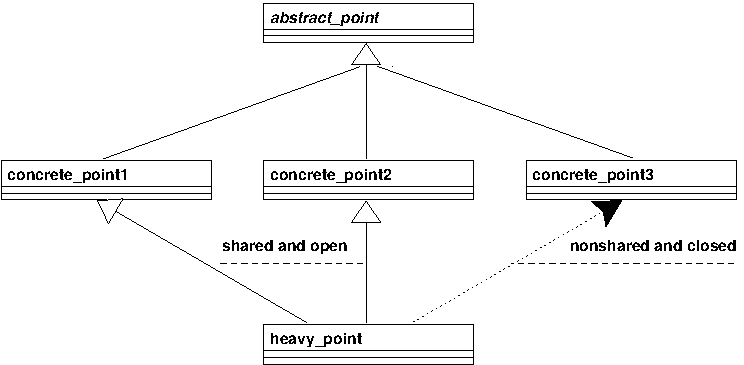
\includegraphics{heavy.pdf}}
\end{center}
\caption{A complex reuse scenario}
\label{F:heavy}
\end{figure}



%%%%%%%%%%%%%%%%%%%%%%%%%%%%%%%%%%%%%%%%%%%%%%%%%%%%%%%%%%%%%%%%%%%%%%%%%%%%%
%%%%%%%%%%%%%%%%%%%%%%%%%%%%%%%%%%%%%%%%%%%%%%%%%%%%%%%%%%%%%%%%%%%%%%%%%%%%%
%%%%%%%%%%%%%%%%%%%%%%%%%%%%%%%%%%%%%%%%%%%%%%%%%%%%%%%%%%%%%%%%%%%%%%%%%%%%%



We are going to work through a scenario, where a class @heavy_point@
is constructed from three different concrete subclasses of
@abstract_point@. The first two concrete points will be shared in the
resulting heavy point, because we leave open the recursive knot. The
third concrete point does not participate in the open recursion; so it
is not shared. See Fig.~\ref{F:heavy} for an overview.

The object template for heavy points starts as follows:

\begin{code}
 heavy_point x_init color self =
  do
     super1 <- concrete_point1 x_init self
     super2 <- concrete_point2 x_init self
     super3 <- mfix (concrete_point3 x_init)
     ... -- to be continued
\end{code}

That is, we bind all ancestor objects for subsequent reference. We
pass @self@ to the first two points, which participate in open
recursion, but we fix the third point in place. (So the first two
classes are reused in the sense of inheritance, while the third class
is reused in the sense of object composition instead.)  A heavy point
carries @print@ and @moveX@ methods that delegate corresponding
messages to all three points:

\begin{code}
     ... -- continued from above
     let myprint = do
                      putStr "super1: "; (super1 # print)
                      putStr "super2: "; (super2 # print)
                      putStr "super3: "; (super3 # print)
     let mymove  = ( \d -> do
                              super1 # moveX $ d
                              super2 # moveX $ d
                              super3 # moveX $ d )
     return 
       $    print  .=. myprint
      .*.   moveX  .=. mymove
      .*.   emptyRecord
     ... -- to be continued
\end{code}

The three points, with all their many fields and methods, contribute
to the heavy point by means of left-biased union on records, which is
denoted by ``@.<++.@'' below:

\begin{code}
     ... -- continued from above
      .<++. super1
      .<++. super2
      .<++. super3
\end{code}

Here is a demo:

\begin{code}
 myDiamondOOP =
  do 
     p <- mfix (heavy_point 42 "blue")
     p # print -- All points still agree!
     p # moveX $ 2
     p # print -- The third point lacks behind!
\end{code}
%%% $

\begin{code}
 ghci> myDiamondOOP
 super1: 42
 super2: 42
 super3: 42
 super1: 46
 super2: 46
 super3: 44
\end{code}

For the record, in OCaml, the rules for multiple inheritance are as
follows. Only the last definition of a method is kept: the
redefinition in a subclass of a method that was visible in the parent
class overrides the definition in the parent class. Previous
definitions of a method can be reused by binding the related ancestor
using a special \ldots @as@ \ldots notation. The bound name is said to
be a pseudo value identifier that can only be used to invoke an
ancestor method.

Other rules and notations exist for Eiffel, C++, and so on. OOHaskell
allows to implement different rules because of the programmability of
the OO type-system aspects. 



%%%%%%%%%%%%%%%%%%%%%%%%%%%%%%%%%%%%%%%%%%%%%%%%%%%%%%%%%%%%%%%%%%%%%%%%%%%%%
%%%%%%%%%%%%%%%%%%%%%%%%%%%%%%%%%%%%%%%%%%%%%%%%%%%%%%%%%%%%%%%%%%%%%%%%%%%%%
%%%%%%%%%%%%%%%%%%%%%%%%%%%%%%%%%%%%%%%%%%%%%%%%%%%%%%%%%%%%%%%%%%%%%%%%%%%%%



\subsection{Typing techniques}

In OOHaskell, one may avoid type annotations and explicit coercions
most of them time. We will now discuss those OOHaskell programming
idioms that can benefit from type annotations and coercion, or that
even require them.



%%%%%%%%%%%%%%%%%%%%%%%%%%%%%%%%%%%%%%%%%%%%%%%%%%%%%%%%%%%%%%%%%%%%%%%%%%%%%%%
%%%%%%%%%%%%%%%%%%%%%%%%%%%%%%%%%%%%%%%%%%%%%%%%%%%%%%%%%%%%%%%%%%%%%%%%%%%%%%%
%%%%%%%%%%%%%%%%%%%%%%%%%%%%%%%%%%%%%%%%%%%%%%%%%%%%%%%%%%%%%%%%%%%%%%%%%%%%%%%



\subsubsection{Narrow to least upper bound}

Subtyping polymorphism in OOHaskell is basically based on @HasField@
constraint satisfaction. That is, a function (a method) that takes an
object as argument constrains the argument type in terms of the
required fields. Naturally, any object with \emph{additional} fields
will be admitted immediately. (We oversimplify by not talking about
methods that add fields.) Such @HasField@ constraint subsumption
implies that narrowing (`up-casting') is normally
unnecessary.\footnote{We prefer the term
\emph{narrow} over \emph{up-cast}, as to emphasise the act of
restricting the interface of an object, as opposed to walking up an
explicit inheritance hierarchy.}

\oleg{Mention the following here? The important difference of our 
polymorphism (which we share with OCaml and ML-ART) and polymorphism
in C++ etc. In the former, an object can be \emph{implicitly} coerced
to an object of any of its super-classes. One may even think that an
object is polymorphic itself (has types of all of its super-classes,
simultaneously) but functions that take objects are mono-morphic.
In OCaml and OOHaskell, it is the other way around: object are
mono-morphic and there is no implicit upcasting. All upcasts must be
explicit. However, functions that process objects can be polymorphic
and can process objects of several tupes. So, the upcasting are
often not needed. We do need the implicit upcasting when we put
objects in a homogeneous list however.}


Narrowing may be necessary if the programmer wants to inform the
Haskell type system about Haskell-based type
\emph{equality} as opposed to OOHaskell subtyping subsumption. 
The shapes examples involved narrowing of that kind:

\begin{code}
 myOOP = do
            s1 <- mfix (rectangle (10::Int) (20::Int) 5 6)
            s2 <- mfix (circle (15::Int) 25 8)
            let scribble = consLub s1 (consLub s2 nilLub)
            ... and so on ...
\end{code}

This code fragment describes the construction of a subtype-polymorphic
collection, @scribble@, with shapes of different kinds. In order to
use a normal, homogeneous Haskell list, one is required to establish
Haskell-based type equality for all elements. The narrow operation
@hLubNarrow@ maps a heterogeneous list to a homogeneous list. The
@hLubNarrow@ operation is the generalization of @lubNarrow@, which is
the least-upper bound (LUB) narrowing operation for pairs:

\begin{code}
 -- LUB narrow heterogeneous lists
 class  HLubNarrow l e | l -> e
  where hLubNarrow :: l -> [e]
\end{code}

\begin{code}
 -- LUB narrowing just for a pair
 class  LubNarrow a b c | a b -> c
  where lubNarrow :: a -> b -> (c,c)
\end{code}

We will explain the @lubNarrow@ operation in some detail. That is,
given two values (presumably records) of types @a@ and @b@, this
operation returns a pair of narrowed values, both of type @c@, while
@c@ is supposed to be the least-upper bound in the sense of structural
subtyping. (In principle, we may consider both width and depth
subtyping; cf.\ Sec.~\ref{S:deep}.) The specification of the
@lubNarrow@ operation nicely illustrates the capability of the
OOHaskell setup to `program' OO type-system aspects. We exploit the
type-level reflection on \HList\ records to define narrowing. The
following specification is tuned for readibility and simplicity. (For
instance, it does not cope with deep subtyping.)

\begin{code}
 instance ( HZip la va a
          , HZip lb vb b
          , HTIntersect la lb lc
          , H2ProjectByLabels lc a c aout
          , H2ProjectByLabels lc b c bout
          , HRLabelSet c
          )
       => LubNarrow (Record a) (Record b) (Record c)
  where
   lubNarrow ra@(Record a) rb@(Record b) =
      ( hProjectByLabels lc ra
      , hProjectByLabels lc rb
      )
    where
     lc = hTIntersect la lb
     (la,_) = hUnzip a
     (lb,_) = hUnzip b
\end{code}

That is, given two records @ra@ and @rb@, we compute the intersection
@lc@ of their labels @la@ and @lb@ such that we can subsequently
project both records to this shared label set.



%%%%%%%%%%%%%%%%%%%%%%%%%%%%%%%%%%%%%%%%%%%%%%%%%%%%%%%%%%%%%%%%%%%%%%%%%%%%%%%
%%%%%%%%%%%%%%%%%%%%%%%%%%%%%%%%%%%%%%%%%%%%%%%%%%%%%%%%%%%%%%%%%%%%%%%%%%%%%%%
%%%%%%%%%%%%%%%%%%%%%%%%%%%%%%%%%%%%%%%%%%%%%%%%%%%%%%%%%%%%%%%%%%%%%%%%%%%%%%%



\subsubsection{Narrow to a fixed type}

Looking back at the shapes example, we note that the use of
@hLubNarrow@ is neither clearly an explicit nor an implicit coercion.
It is \emph{explicit} in so far that we must perform narrowing in
order to assure Haskell-based type equality; it is \emph{implicit} in
so far that we did not need to specify the target type for
narrowing. Instead we presumed that the LUB is determined by the
operation itself. We may also perform fully explicit narrowing to a
fixed, programmer-defined upper bound type:

\begin{Verbatim}[fontsize=\small,commandchars=\\\{\}]
 let scribble :: [Shape Int]
     scribble = [narrow s1, narrow s2]
\end{Verbatim}

In this code fragment, applications of @narrow@ prepare the shape
objects for insertion into the homogeneous Haskell list. For brevity,
we only provide the type for the @narrow@ operation. Its specification
uses the same kind of projection on records as @lubNarrow@.

\begin{code}
 class  Narrow a b
 where  narrow :: Record a -> Record b
 -- extract those label-value pairs from "a" that are requested by "b"
\end{code}

Here is the @Shape@ type, which `drives' narrowing in the example:

\begin{code}
 -- The Shape interface
 type Shape a = Record (  GetX    :=: IO a
                      :*: GetY    :=: IO a
                      :*: SetX    :=: (a -> IO ())
                      :*: SetY    :=: (a -> IO ())
                      :*: MoveTo  :=: (a -> a -> IO ())
                      :*: RMoveTo :=: (a -> a -> IO ())
                      :*: Draw    :=: IO ()
                      :*: HNil )
\end{code}

We note that we have included the virtual @draw@ operation because it
is a part of the interface that is used in the loop over
@scribble@. For comparison we note that narrowing in the context of
constructing subtype-polymorphic collections is \emph{fully implicit}
in the C++ code from which we started~---~but must be \emph{fully
explicit} in OCaml. (OCaml has no counterpart to OOHaskell's
@hLubNarrow@.)

We will see more applications of @narrow@ in subsequent sections.



%%%%%%%%%%%%%%%%%%%%%%%%%%%%%%%%%%%%%%%%%%%%%%%%%%%%%%%%%%%%%%%%%%%%%%%%%%%%%%%
%%%%%%%%%%%%%%%%%%%%%%%%%%%%%%%%%%%%%%%%%%%%%%%%%%%%%%%%%%%%%%%%%%%%%%%%%%%%%%%
%%%%%%%%%%%%%%%%%%%%%%%%%%%%%%%%%%%%%%%%%%%%%%%%%%%%%%%%%%%%%%%%%%%%%%%%%%%%%%%



\subsubsection{Self-returning methods}

The type of `self' is known to be a difficult issue in the encoding of
typed objects; cf.\ \cite{AC96,PolyTOIL} for some advanced
treatments. (A self-returning method is a method whose result type is
the type of self or is constructed from the type of self.) In
OOHaskell, a restricted type for `self' can be provided easily. That
is, we do not allow to return just polymorphic self itself, but we
require from the programmer to narrow self to a fixed interface.

The following attempt to define a method @me@ that returns @self@ will
not type check (once we @mfix@ the generator) since it would imply a
recursive type for the type of @self@. We recall that recursive types
are not admitted by Haskell (but see Sec.~\ref{S:nominal} for a
resolution).

\begin{code}
 self_returning_point (x_init::a) self =
   do
      super <- printable_point x_init self
      returnIO
          $  me .=. self
         .*. super
\end{code}
%%% $

This is, of course, just an illustrative example. A more principled
example for a self-returning method would be a \emph{clone}
method. The following variation allows us to return (part of) @self@:

\begin{code}
 self_returning_point (x_init::a) self =
   do
      super <- printable_point x_init self
      returnIO
          $  me .=. (narrow self :: PPInterface a)
         .*. super
\end{code}
%%% $

To this end, we explicitely identify the interface for printable
points:

\begin{code}
 type PPInterface a
    = Record (  GetX  :=: IO a
            :*: MoveX :=: (a -> IO ())
            :*: Print :=: IO ()
            :*: HNil )
\end{code}

The explicit narrowing approach can be compared to the situation in
C++ or Java in so far that the return type of a method must be
\emph{explicitly declared} in these languages. We must note a
limitation of the presented @narrowing@ approach: all record
components that do not occur in the interface are chopped off in an
irreversible manner.

\ralf{Oleg! What to do about it?}
\oleg{Say that these components become private. That is quite
  reasonable.}

\ralf{
Oleg, see commented-out stuff below. What to do with it?
Do we need it? I would definitely be in favour of saying something
useful about other treatments of self's type in PT94 or
elsewhere. Such discussion may end up in the related work section 
of course.}
\oleg{I'd suggest just drop it. The references at the beginning of the
section should suffice.}

\begin{comment}

This is what Oleg had to say: In PT94, they use existential to
implement self without the recursive types, to break the
recursion. self has the type like OpaqueShape below -- or
OpaqueRectange for rectangle, etc.  BTW, we should use that fact to
relate to returning of self in our encoding. One can't return self,
only a restriction of self to the class and its superclasses.

\end{comment}



%%%%%%%%%%%%%%%%%%%%%%%%%%%%%%%%%%%%%%%%%%%%%%%%%%%%%%%%%%%%%%%%%%%%%%%%%%%%%
%%%%%%%%%%%%%%%%%%%%%%%%%%%%%%%%%%%%%%%%%%%%%%%%%%%%%%%%%%%%%%%%%%%%%%%%%%%%%
%%%%%%%%%%%%%%%%%%%%%%%%%%%%%%%%%%%%%%%%%%%%%%%%%%%%%%%%%%%%%%%%%%%%%%%%%%%%%



\subsubsection{Explicit type constraints}

In some cases, it is useful to impose type constraints on arguments of
an object generator, on arguments of a method or on the result type of
a method. We are here interested in type constraints that concern
structural record type. OOHaskell devises type-level narrowing to
this end; no actual coercions are performed at the value
level. OOHaskell's type constraints are akin to C++
\emph{concepts}~\cite{siek05:_concepts_cpp0x}.
As a principled example of OO type constraints, we have chosen to
review the default treatment of virtual methods in OOHaskell, which
indeed can benefit from the use of type constraints.

Quoting from~\cite{OCaml}[\S\,3.4]:

\begin{quote}\itshape\small
``It is possible to declare a method without actually defining it,
using the keyword @virtual@. This method will be provided later in
subclasses. A class containing virtual methods must be flagged
virtual, and cannot be instantiated (that is, no object of this class
can be created). It still defines type abbreviations (treating virtual
methods as other methods.)
\end{quote}

\begin{code}
 class virtual abstract_point x_init =
   object (self)
     val mutable varX = x_init
     method print = print_int self#getX
     method virtual getX : int
     method virtual moveX : int -> unit
   end;;
\end{code}

In C++, one calls such methods \emph{pure} virtual methods and classes
that cannot be instantiated are called abstract. In Java, we can flag
classes as being abstract. In OOHaskell, it is enough to leave the
method undefined.

\begin{code}
 abstract_point x_init self =
   do
      xRef <- newIORef x_init
      returnIO $
           varX   .=. xRef
       .*. print  .=. ( self # getX >>= Prelude.print )
       .*. emptyRecord
\end{code}
%%% $

This class cannot be instantiated with @mfix@ because @getX@ is used
but not defined. The Haskell type system effectively prevents us from
instantiating classes which use methods neither they nor their parents
have defined. There arises the question of the explicit designation of
a method as pure virtual, which would be of particular value in case
the pure virtual does not happen to be used in the class itself.

OOHaskell allows for such explicit designation by means of adding type
constraints to @self@. If we wanted to designate @getX@ and @moveX@ as
pure virtuals of @abstract_point@, then we have enhance the class as
follows:

\begin{code}
 abstract_point (x_init::a) self =
   do
      ... as before ...
 where
  _ = narrow self :: Record (  GetX  :=: IO a
                           :*: MoveX :=: (a -> IO ())
                           :*: HNil )
\end{code}

Again, we use the @narrow@ operation, this time to express a type
constraint. It is important to notice that we narrow at the
\emph{type level} only. That is, the result of narrowing is 
obviously not used (cf.\ ``\_''). However, type-checking
@abstract_point@ (or applications thereof, including fix-point taking)
implies checking the feasibility of narrowing.

One may argue that normal type annotation would be sufficient for 
the imposition of type constraints. However, type annotations would
require from the programmer to identify the complete structural type
of @self@. Also, a normal type annotation would use the normal
Haskell-based type equality to check the constraint.  This would imply
that the structural type in the annotation and the actual structural
type of @self@ would need to be \emph{literally} the same~---~without
any variance regarding order of record components, without any
variance regarding deep subtyping (cf.\ Sec.~\ref{S:deep}).
\oleg{Another approach: signature. Their, HasField constraints don't
  have to be complete, and can be given in any order. Alas, we have to
  specify the return type completely then. Our approach here is
  tantamount to a partial signature.}


%%%%%%%%%%%%%%%%%%%%%%%%%%%%%%%%%%%%%%%%%%%%%%%%%%%%%%%%%%%%%%%%%%%%%%%%%%%%%
%%%%%%%%%%%%%%%%%%%%%%%%%%%%%%%%%%%%%%%%%%%%%%%%%%%%%%%%%%%%%%%%%%%%%%%%%%%%%
%%%%%%%%%%%%%%%%%%%%%%%%%%%%%%%%%%%%%%%%%%%%%%%%%%%%%%%%%%%%%%%%%%%%%%%%%%%%%



\subsubsection{Nominal types}
\label{S:nominal}

By default, OOHaskell's object types engage in structural subtype
polymorphism~---~just as in OCaml. Many other OO languages prefer
nominal classes. It turns out that we can easily establish nominal
disctinctions. In fact, certain OO programming scenarios require
nominal types. Most notably, we \emph{must} introduce nominal types in
case we deal with recursive object types.  (In such cases, the nominal
type (``newtype'') serves as iso-recursive type. A type system with
equi-recursive types would be slightly more convenient in this
respect, while it would injure type inference at the same time.)
\oleg{injure type inference is perhaps less precise. Say that
  recursive types have known drawbacks, enough to avoid them in
  Haskell. Perhaps ref to Hughes' message on Haskell-list and the fact
OCaml by default restricts recursive types for object types only.
For more detail, see the comment in the TeX source below.}

\begin{comment}
Such an extension (equi-recursive types)
 to Haskell was also debated and then rejected
because it will make type-error messages nearly
useless~\cite{Hughes02}. There is an alternative technique for
encoding objects: eschew recursive types in favour of existential
quantification~\cite{PT94}. Unfortunately, the involved higher-ranked
types can not be inferred anymore. Explicit signatures were required,
which, in practical terms, means that the user must explicitly
enumerate all virtual methods in the signature of any function that
operates on an object. This technique cannot be used in OOHaskell
because we would like OO programming to be easy to use, first, by Haskell
programmer. That is, we ought to preserve type inference for functions
that use objects. Type inference is the great advantage of Haskell and
ML and is worth fighting for. 

\end{comment}

We illustrate nominal types with uni-directionally linked dynamic
lists. The interface of such list objects comprises methods that also
return list objects. This is the way recursion enters the scene, and
therefore a newtype is needed to represent the interface for linked
dynamic lists:

\begin{code}
 -- The structural interface type
 type ListInterface a =
      Record (     (Proxy IsEmpty  , IO Bool)
               :*: (Proxy GetHead  , IO a)
               :*: (Proxy GetTail  , IO (ListObj a))
               :*: (Proxy SetHead  , a -> IO ())
               :*: (Proxy InsHead  , a -> IO (ListObj a))
               :*: HNil )
\end{code}

\begin{code}
 -- The nominal object type
 newtype ListObj a =
         ListObj (ListInterface a)
\end{code}

There is basically just one issue that we need to resolve before we
can leverage OOHaskell idioms on nominal types. That is, we need to
make sure that method invocation continues to work for the nominal
types. To this end, we have to complement each newtype by a @HasField@
instance (for the ``@#@'' operation) as follows:

\begin{code}
 instance HasField l (ListInterface a) v =>
          HasField l (ListObj a) v
   where
   hLookupByLabel l (ListObj x) = hLookupByLabel l x
\end{code}

This instance simply forwards the look-up operation to the wrapped
object type. One may want to avoid coding such an instance for each
nominal type. It is indeed trivial to automate the derivation of these
forwarding instances by Template Haskell~\cite{SPJ02} or
DrIFT~\cite{Winstanley97}.

We consider two classes~---~one for the empty list, another for the
non-empty list. (This split is not essential; we could also implement
the same behaviour with just one class.) The @nil_class@ fails for all
getters, but it reports the status to be empty, and it also allows for
the insertion of a head:

\begin{code}
 nil_class (_::Proxy a) self
  = returnIO
      $  isEmpty  .=. returnIO True
     .*. getHead  .=. ((failIO "No head!")::IO a)
     .*. getTail  .=. ((failIO "No tail!")::IO (ListObj a))
     .*. setHead  .=. const ((failIO "No head!")::IO ())
     .*. insHead  .=. reusableInsHead self
     .*. emptyRecord
\end{code}
%%% $

The reusable insert operation constructs a new object of the @cons_class@:

\begin{code}
 reusableInsHead self (head::a)
  = do 
       newCons <- mfix (cons_class head self)
       returnIO ((ListObj newCons)::ListObj a)
\end{code}

The @cons_class@ succeeds for the full interface. Each cons object
holds a reference for the head, which is accessed by @getHead@ and
@setHead@.

\begin{code}
 cons_class head tail self
  = do
       hRef <- newIORef head
       returnIO
         $  isEmpty .=. returnIO False
        .*. getHead .=. readIORef hRef
        .*. getTail .=. returnIO (ListObj tail)
        .*. setHead .=. writeIORef hRef
        .*. insHead .=. reusableInsHead self
        .*. emptyRecord
\end{code}
%%% $

Normal OOHaskell programming can commence on nominally typed lists.
The following recursive function prints a given (nominal) list object.
The various method invocations access nominal objects or even return
such objects.

\begin{code}
 printList aList
  = do
       empty <- aList # isEmpty
       if empty
         then putStrLn ""
         else ( do 
                   head <- aList # getHead
                   putStr $ show head
                   tail <- aList # getTail
                   putStr " "
                   printList tail
              )
\end{code}
%%% $



%%%%%%%%%%%%%%%%%%%%%%%%%%%%%%%%%%%%%%%%%%%%%%%%%%%%%%%%%%%%%%%%%%%%%%%%%%%%%%%
%%%%%%%%%%%%%%%%%%%%%%%%%%%%%%%%%%%%%%%%%%%%%%%%%%%%%%%%%%%%%%%%%%%%%%%%%%%%%%%
%%%%%%%%%%%%%%%%%%%%%%%%%%%%%%%%%%%%%%%%%%%%%%%%%%%%%%%%%%%%%%%%%%%%%%%%%%%%%%%



\section{Discussion of the OOHaskell sandbox}
\label{S:discuss}


\ralf{I need to write an intro eventually.}

Here's the phrase (mentioned below in the ML-ART section, too:

\oleg{Ralf, note the phrase: Remy's ML-ART paper, page 15
(beginning of Section 3.7):``The same message print can be sent to
  points and colored points. However, both of them have incompatible
  types and can never be stored in the same list. Some languages with
  subtyping allow this set-up. They would take the common interface
  of all objects that are mixed in the list as the interface of any
  single object of the list.''
  Isn't what our Stynamic subtyping and even lub were doing?
}

So, OOHaskell can emulate those languages with subtyping, mentioned in
Remy's quote, to some extent. So, OOHaskell indeed supports a good
measure of experimentation -- all without changing the type system and
the compiler.


%%%%%%%%%%%%%%%%%%%%%%%%%%%%%%%%%%%%%%%%%%%%%%%%%%%%%%%%%%%%%%%%%%%%%%%%%%%%%
%%%%%%%%%%%%%%%%%%%%%%%%%%%%%%%%%%%%%%%%%%%%%%%%%%%%%%%%%%%%%%%%%%%%%%%%%%%%%
%%%%%%%%%%%%%%%%%%%%%%%%%%%%%%%%%%%%%%%%%%%%%%%%%%%%%%%%%%%%%%%%%%%%%%%%%%%%%



\subsection{Clarity of inferred types}

One may wonder about the clarity of inferred types. Can they be used
as means of program understanding? Do we need dedicated support to
make the inferred types more accessible?

Let us infer the result of constructing a colored point:
 
\begin{code}
 ghci6.4> :t mfix $ colored_point (1::Int) "red"
 mfix $ colored_point (1::Int) "red" ::
        IO (Record 
            (HCons (Proxy GetColor, IO String)
             (HCons (Proxy VarX, IORef Int)
              (HCons (Proxy GetX, IO Int)
               (HCons (Proxy MoveX, Int -> IO ())
                (HCons (Proxy Print, IO ())
                 HNil))))))
\end{code} 

We think that this type is pretty readable, even though it reveals the
underlying representation of records (as a heterogeneous list of
label-value pairs), and it also gives away the proxy-based model for
labels.  We may hope for a future Haskell implementation whose
customisable `pretty printer' for types would present the result of
type inference perhaps as follows:

\begin{code}
 ghci> :t mfix $ colored_point (1::Int) "red"
 mfix $ colored_point (1::Int) "red" ::
        IO ( Record (
               GetColor :=: IO String
           :*: VarX     :=: IORef Int
           :*: GetX     :=: IO Int
           :*: MoveX    :=: Int -> IO ()
           :*: Print    :=: IO ()
           :*: HNil ))
\end{code} 

We had resolved all polymorphism in the previous example. Also, the
recursive knot was tied. Let us consider type inference for the case
of more polymorphic, more parametric expressions. Here is the
(pretty-printed) type of class @colored_point@:

\begin{code}
 ghci> :t colored_point
 ( Num a
 , HasField GetX r (IO a1)
 , Show a1
 ) => a
   -> String
   -> r
   -> IO ( Record (
             GetColor :=: IO String
         :*: VarX     :=: IORef a
         :*: GetX     :=: IO a
         :*: MoveX    :=: a -> IO ()
         :*: Print    :=: IO ()
         :*: EmptyRecord ))
\end{code}

That is, the type of the constructor essentially lists all the fields
of an object, both new and inherited. Assumptions about @self@ are
expressed as constraints on the type variable @r@. The constructor
@colored_point@ refers to @getX@ (through @self@), and hence this
reference implies a constraint of the form
@HasField@~@GetX@~@r@~@(IO@~@a1)@.

We note the polymorphism in the coordinate type for the point; cf.\
@a@ (and @a1@). Since arithmetic is performed on @GetX@, this implies
bounded polymorphism: only @Num@ types are permitted. Interestingly,
type inference does not infer the fact that @a@ and @a1@ eventually
must be the same. (@r@ with the @HasField GetX r (IO a1)@ constraint
is part of the result record whose @GetX@ component is said to be of
type @a@.)  This equality is not inferred because we have not (yet)
taught the type system about the law that record extension preserves
the type of previous components.

We must admit that we have assumed a \emph{relatively} eager instance
selection in the previous session. The hugs implementation of Haskell
is (more than) eager enough. The recent versions of GHC have become
more and more lazy. In a session with contemporary GHC (6.4) we would
additionally see the following constraints, which deal with the
uniqueness of label sets as they are encountered during record
extension:

\begin{Verbatim}[fontsize=\small,commandchars=\\\{\}]
 HRLabelSet (HCons (Proxy MoveX, a -> IO ())
            (HCons (Proxy Print, IO ()) HNil)),
 \cmt{likewise for} MoveX, Print, GetX
 \cmt{likewise for} MoveX, Print, GetX, VarX
 \cmt{likewise for} MoveX, Print, GetX, VarX, GetColor
\end{Verbatim}
 
Inspection of the @HRLabelSet@ instances would reveal that these
constraints are all satisfied, no matter how the type variable @a@ is
instantiated. No ingenuity is required. A simple form of strictness
analysis is sufficient. Alas, GHC is consistently lazy in resolving
even such constraints.

We think that the type without the @HRLabelSet@ constraints looks very
reasonable. The type explicitly lists all the fields and the types of
their values. Because the type lists both the new fields and all
inherited fields, the type could even be used for the simple
implementation of a class browser in an IDE. (The class browser does
not need to figure out the set of all methods in a class by itself:
the compiler has already done that, and expressed in the type.)

We must mention that the issue of the object types, as inferred vs. as
they are actually shown to the user existed for OCaml, and it has been
resolved as we hypothesised it could for Haskell. Although objects
types shown by OCaml are quite concise, that has not always been the
case. In the {ML-ART} system, the predecessor of OCaml with no
syntactic sugar~\cite{ML-ART} (Section 3):

\begin{quote}\small
``Objects have anonymous, long, and often recursive
types that describe all methods that the object can receive. Thus, we
usually do not show the inferred types of programs in order to
emphasize object and inheritance encoding rather than typechecking
details. This is quite in a spirit of ML where type information is
optional and is mainly used for documentation or in module
interfaces. Except when trying top-level examples, or debugging, the
user does not often wish to see the inferred types of his programs in
a batch compiler.''
\end{quote}



%%%%%%%%%%%%%%%%%%%%%%%%%%%%%%%%%%%%%%%%%%%%%%%%%%%%%%%%%%%%%%%%%%%%%%%%%%%%%
%%%%%%%%%%%%%%%%%%%%%%%%%%%%%%%%%%%%%%%%%%%%%%%%%%%%%%%%%%%%%%%%%%%%%%%%%%%%%
%%%%%%%%%%%%%%%%%%%%%%%%%%%%%%%%%%%%%%%%%%%%%%%%%%%%%%%%%%%%%%%%%%%%%%%%%%%%%



\subsection{Clarity of type errors}

\ralf{This section is a big mess, but I know how to fix.
I also want to show an Occurs check error and perhaps something
else. Bottomline: be honest.}

Due to the underlying foundation of OOHaskell to employ
type-class-based programming, there is a risk that type errors may
just become too complex. 

This specific class cannot be instantiated with @mfix@ because @getX@
is used but not defined. If we tried to take the fix-point, Haskell's
type checker (GHC 6.4) offers the following error message:

\begin{code}
 ghci> let x = mfix (abstract_point 7)
 No instance for (HasField (Proxy GetX) HNil (IO a))
   arising from use of `abstract_point' at <interactive>:1:14-27
 Probable fix:
   add an instance declaration for (HasField (Proxy GetX) HNil (IO a1))
 In the first argument of `mfix', namely `(abstract_point 7)'
 In the definition of `x': x = mfix (abstract_point 7)
\end{code}

We think that the error message is concise and to the point. The
message succinctly lists just the missing field. (The suggested
`probable fix' is not really helpful.) In the next sections, we will
show a type error, which is less clear than the one at hand.

We have to admit that the verbosity of OOHaskell error messages may
occassionally compare to error messages in C++ template instantiation,
which can be immensely verbose, spanning several dozens of packed
lines, and yet boost and similar C++ libraries, which extensively use
templates, are gaining momentum. In general, the clarity of error
messages is undoubtedly an area that needs more research, and such
research is being done~\cite{SSW04}, which we or compiler writers may
take advantage of.

It is worth noting that an instantiation test for the annotated
@abstract_point@ class will now lead to a more overwhelming type
error:

\begin{code}
 ghci> let x = mfix (abstract_point 7)
 No instance for (HExtract HNil (Proxy GetX) (IO a),
                  HExtract HNil (Proxy MoveX) (a -> IO ()),
                  HasField (Proxy GetX) HNil (IO a1))
   arising from use of `abstract_point' at <interactive>:1:14-27
 Probable fix: ...
 In the first argument of `mfix', namely `(abstract_point 7)'
 In the definition of `x': x = mfix (abstract_point 7)
\end{code}

That is, in addition to unsatisfiable @HasField@ constraint, due to
the attempted invocation of @getX@, we also see two constraint
failures that are implied by the added constraint.  The trouble is
that type-system implementation details leak through. That is, the
failed constraint
%
\[@HExtract HNil (Proxy GetX) (IO a)@\]
%
indicates that the look-ups of the narrowing operation reached the
`end' of the record type (cf.\ @HNil@), while the required field with
the label @getX@ was not found. One might also argue that two of the
three failed constraints should be summarised as single type error:
%
\begin{center}
\begin{tabular}{l}
@HExtract HNil (Proxy GetX) (IO a)@\\
@HasField (Proxy GetX) HNil (IO a1)@
\end{tabular}
\end{center}
%
Both failed constraints basically express the absence of a required
field. More generally, type errors will be improved if constraint
failures can be translated to constraint-specific error messages, and
if multiple constraint failures could be reduced before exposing them
as type errors to the programmer.



%%%%%%%%%%%%%%%%%%%%%%%%%%%%%%%%%%%%%%%%%%%%%%%%%%%%%%%%%%%%%%%%%%%%%%%%%%%%%
%%%%%%%%%%%%%%%%%%%%%%%%%%%%%%%%%%%%%%%%%%%%%%%%%%%%%%%%%%%%%%%%%%%%%%%%%%%%%
%%%%%%%%%%%%%%%%%%%%%%%%%%%%%%%%%%%%%%%%%%%%%%%%%%%%%%%%%%%%%%%%%%%%%%%%%%%%%



\subsection{Subtype-polymorphic collections}

\ralf{I am going to work through once more. Looks almost fine.}

We already have seen two reasonable approaches for the construction of
a subtype-polymorphic collection, as required in the shapes example:
least-upper bound casting and element-wise casting. When we discussed
non-OOHaskell encodings, we had also considered two additional options:
%
\begin{itemize}
\item We use \HList's heterogeneous lists.
\item We make the list elements opaque (through ``$\exists$'').
\end{itemize}
%
These two apparant approaches had their problems even for the normal,
non-extensible Haskell records. In the combination with OOHaskell (and
its extensible records), these two approaches are definitely not
attractive, as we will show.

In first case, we construct the scribble list as follows:

\begin{code}
 let scribble = s1 `HCons` (s2 `HCons` HNil)
\end{code}

According to Sec.~\ref{S:hetero}, we map over the list as follows:

\begin{Verbatim}[fontsize=\small,commandchars=\\\{\}]
 hMapM_ (\undefined::ScribbleBody) scribble
\end{Verbatim}

The corresponding @Apply@ instance must be constrained as follows:

\begin{code}
instance ( HasField (Proxy Draw) r (IO ())
         , HasField (Proxy RMoveTo) r (Int -> Int -> IO ())
         )
      => Apply FunOnShape r (IO ())
  where
    apply _ x = do
                   x # draw
                   (x # rMoveTo) 100 100
                   x # draw
\end{code}

That is, we list the \emph{method-access constraints} (for ``\#'',
i.e., @HasField@) in the @Apply@ instance. Haskell's type-class system
requires us to provide proper bounds for the instance. One might argue
that the form of these constraints strongly resembles the method types
listed in the class type @Shape@. So one might wonder whether we can
somehow use the full class type, @Shape@, in order to constrain the
instance.  Haskell will not let us do that in any reasonable
way. Constraints are not first-class citizens in Haskell; we cannot
compute them from types or type proxies~---~unless we were willing to
rely on heavy encoding or advanced syntactic sugar. So we are doomed
to manually infer such method-access constraints for each such piece
of polymorphic code.

The existential quantification approach falls short for essentially
the same reason. Assumming a suitable existential envelope and
following Sec.~\ref{S:exists}, we construct the subtype-polymorphic
collection as follows:

\begin{code}
 let scribble = [ HideShape s1, HideShape s2 ]
\end{code}

The declaration of the existential type depends on the function that
we want to apply to the opaque data. In our case, we can use the
normal @mapM_@ function again; we only need to unwrap the @HideShape@
constructor prior to method invocations:

\begin{code}
 mapM_ ( \(WrapShape shape) -> do
             shape # draw
             (shape # rMoveTo) 100 100
             shape # draw )
         scribble
\end{code}

These operations have to be anticipated in the type bound for the
envelope:

\begin{Verbatim}[fontsize=\small,commandchars=\\\{\}]
 data OpaqueShape =
  forall x. ( HasField (Proxy Draw) x (IO ())
            , HasField (Proxy RMoveTo) x (Int -> Int -> IO ())
            ) => HideShape x
\end{Verbatim}

It becomes evident that this result agrees with the heterogeneity
technique in terms of encoding efforts. In both cases, we need to
identify type-class constraints that correspond to the (potentially)
polymorphic method invocations. This is a show stopper. So the use of
explicit casting (@narrow@) or more implicit LUB construction
(@hLubNarrow@) is clearly to be preferred.



%%%%%%%%%%%%%%%%%%%%%%%%%%%%%%%%%%%%%%%%%%%%%%%%%%%%%%%%%%%%%%%%%%%%%%%%%%%%%
%%%%%%%%%%%%%%%%%%%%%%%%%%%%%%%%%%%%%%%%%%%%%%%%%%%%%%%%%%%%%%%%%%%%%%%%%%%%%
%%%%%%%%%%%%%%%%%%%%%%%%%%%%%%%%%%%%%%%%%%%%%%%%%%%%%%%%%%%%%%%%%%%%%%%%%%%%%



\subsection{Width and depth subtyping}
\label{S:deep}

\oleg{we need to mention somewhere the important difference of our 
polymorphism (which we share with OCaml and ML-ART) and polymorphism
in C++ etc. In the former, an object can be \emph{implicitly} coerced
to an object of any of its super-classes. One may even think that an
object is polymorphic itself (has types of all of its super-classes,
simultaneously) but functions that take objects are mono-morphic.
In OCaml and OOHaskell, it is the other way around: object are
mono-morphic and there is no implicit upcasting. All upcasts must be
explicit. However, functions that process objects can be polymorphic
and can process objects of several tupes. So, the upcasting are
often not needed. We do need the implicit upcasting when we put
objects in a homogeneous list however.}

As common \cite{Poll97} we take subtyping to mean type
substitutability: Specifically, we call the object type @S@ to be a
subtype of the object type @T@ if in any well-typed program @P@ the
typing of method invocation operators is preserved upon replacing
objects of type @T@ with objects of type @S@. This notion of subtyping
(to be distinguished from behavioral subtyping, also know as Liskov
Substitution Principle \cite{LiskovW94}) is related to subclassing and
is consistent with the OO practice (ref to Cook, Inheritance not
Subtyping?). This notion of subtyping is formalized in the subtyping
relation of System $F_{<=}$ \cite{Poll97}.

Subtyping is enabled by the type of the method invocation
operator @#@. To be more concrete, the function @\r -> r # getX@ has
the inferred type @HasField (Proxy GetX) r v => r -> v@, which is
polymorphic. The function will accept any object (synonymous with
Record in OOHaskell) @r@ provided that it has the method labelled
@GetX@ whose type matches function's desired return type @v@.

We can therefore define a so-called width-subtyping relation \cite{Poll97},
whereupon an object of type @S@ is a subtype of @T@ if the record @S@
has all the fields of @T@ (of the same name, of the same type).
The \HList\ library already provides this subtyping relation,
@Record.SubType@. It is easy to see that if @SubType S T@ holds for
some record types @S@ and @T@, then substituting an object of type @S@
for an object of type @T@ preserves the typing of every occurrence of
@#@ in a program. There will be no missing methods and no method
will be of a wrong type.

\begin{comment}
The width-subtyping is not the only possible subtyping relation in
OOHaskell. We can introduce a more liberal method invocation operation
@##@ so that @\r -> r ## getX@ has the type
@(HasField (Proxy GetX) r v', DeepNarrow v' v) => r -> v@


The relation @DeepNarrow@ is represented by a contraint and the
corresponding convertion function. It is easy to see that @##@ is just
the old @#@ composed with the convertion function. Because the
converstion function is idempotent, many occurrence of the convertion
function can be eliminated (elided) in actual programs. In C++ and
Java, the conversion is implicit. 
\end{comment}

The width subtyping is not the only subtyping relation consistent with
the typing of @#@. To make the discussion concrete, let us recall
the example of one-dimensional 
@printable_point@ from Section~\ref{sec:open-recursion} and its
subclass @colored_point@ from
Section~\ref{sec:single-inheritance:override}. We define a
simple-minded one-dimensional vector class, specified by the beginning
and the end points, which can be accessed by the methods @getP1@ and
@getP2@:
\begin{code}
vector (p1::p) (p2::p) self =
   do p1r <- newIORef p1; p2r <- newIORef p2
      returnIO $
           getP1    .=. readIORef p1r
       .*. getP2    .=. readIORef p2r
       .*. print    .=. do self # getP1 >>= ( # print )
                           self # getP2 >>= ( # print )
       .*. emptyRecord
\end{code}
%% $

The local type annotation @::p@ makes sure that the two points of the
vector have the same type. That type should be the type of an object
responding to the message @print@. Otherwise, the type of the points
is not constrained. That makes the class @vector@ parameterized over
the class of the point. In C++, the analogue of such a class is a 
class \emph{template}. In OOHaskell, we obtain parameterized classes
for free, without any extensions.

We construct two instances of the vector class, @v@ and @cv@
\begin{code}
test1 = do
	p1  <- mfix (printable_point 0)
	p2  <- mfix (printable_point 5)
	cp1 <- mfix (colored_point 10 "red")
	cp2 <- mfix (colored_point 25 "red")
	v  <- mfix (vector p1 p2)
	cv <- mfix (vector cp1 cp2)
	-- ... to be continued
\end{code}
The former is the vector of two printable points; the latter is the
vector of two colored points. The types of @v@ and @cv@ are
obviously different: the type checker will remind us of this fact 
if we try to put both vectors into the same homogeneous list. The
vectors @v@ and @cv@ are not related by the width subtyping: indeed,
both vectors have three methods of the same name. The types of the
method @getP1@ in both vectors are different however. In @v@, the
method @getP1@ has the type @IO PrintablePoint@ whereas in @cv@
the same method has the type @IO ColoredPoint@. The point types 
differ yet are related by the width subtyping.

Despite the fact that @Record.SubType cv v@ does not hold, the type
of @cv@ is a subtype of @v@---a \emph{deep} subtype \cite{Poll97}.
Indeed we can pass either vector to a function such as
\begin{code}
norm v =
    do
    p1 <- v # getP1; p2 <- v  # getP2
    x1 <- p1 # getX; x2 <- p2 # getX
    return (abs (x1 - x2))
\end{code}

so that the above test continued as
\begin{code}
        -- .. continued
	putStrLn "Length of v"
        norm v >>= Prelude.print
	putStrLn "Length of colored cv"
        norm cv >>= Prelude.print
\end{code}
The method access operations within @norm@ remain well-typed no matter
which vector, @v@ or @cv@, we pass to that function.  We attain a
more extensive subtyping relation, which combines the width subtyping
with the depth subtyping \cite{Poll97}: the object type @S@ is a
subtype of @R@ if the record @S@ has all the fields of @R@ whose types
are not necessarily the same but related by subtyping in turn. This
subtyping relation trivially extends to @IO (Record a)@ and 
@t->Record b@ and to the base types. It is the identity on the latter. At
present, we relate functional types by subtyping if the return types
are related by subtyping but the argument types are identical.

We observe that we never had to specifically assert that the types of
two objects are related by width or depth subtyping. This is because
in each and every case, the compiler checks the well-typedness of all
method invocations directly, so no separate subtyping rules are
needed. \oleg{say that in System @F<=@ they need special subsumption
  inference rules?} This is in contrast with C++ where subtyping
relation is asserted as a subclassing declaration.

The only place we have to make subtyping explicit is in explicit
narrowing operations, so we can place, for example, @v@ and @cv@,
into the same homogeneous list. Now we have to write
\begin{code}
	let vectors = [deep'narrow v, deep'narrow cv]
		      `asTypeOf` [v]
\end{code}
where the operation @deep'narrow@ must essentially descend into records and
postfix all ``method returns'' by a narrow operation on the results.
There is no magic about the definition of deep subtyping. It is
essentially just another record operation that is driven by the
structure of method types (We refer to source distribution for
details.)

\oleg{Just a note: deep'narrow is even more destructive than plain
  narrow. deep'narrow not only rebuilds the record but also rebuilds
  the methods. OTH, the union/intersection contraption is not
  destructive and can be adopted for co-variant methods.}


\begin{comment}
Suppose you have a class @cube@ and a subclass @cuboid@, which
overrides one of @cube@'s methods by a version with a co-variant
return type (as in Java 5, for example). Substitutability of cubes by
cuboids does not require any casting effort or otherwise. However, we
can coerce a cuboid to become \emph{exactly} of type cube through a
narrowing operation that involves depth subtyping:

\begin{code}
 testDeep = do
   (cuboid::cuboid) <- mfix (class_cuboid
                         (10::Int) (20::Int) (30::Int))
   cube <- mfix (class_cube (40::Int))
   let cuboids = [cuboid, deep'narrow cube]
   putStrLn "Volumes of cuboids"
   mapM_ (\cb -> handle_cuboid cb >>= print) cuboids
\end{code}
\end{comment}




%%%%%%%%%%%%%%%%%%%%%%%%%%%%%%%%%%%%%%%%%%%%%%%%%%%%%%%%%%%%%%%%%%%%%%%%%%%%%
%%%%%%%%%%%%%%%%%%%%%%%%%%%%%%%%%%%%%%%%%%%%%%%%%%%%%%%%%%%%%%%%%%%%%%%%%%%%%
%%%%%%%%%%%%%%%%%%%%%%%%%%%%%%%%%%%%%%%%%%%%%%%%%%%%%%%%%%%%%%%%%%%%%%%%%%%%%



\subsection{Covariant method arguments}

The subtyping relation of the previous section required that argument
types of functions related by subtyping be the same. That restriction
can be relaxed \cite{AC96}: the function type @R1 -> S1@ is a subtype
of @S2 -> R2@ if @S1@ is a subtype of @R2@ (co-variance) and
@S2@ is a subtype of @R1@ (contra-variance for argument types). For
example, if we extend our @vector@ template of the previous section
with a method @moveO p@ to move the origin of the vector to the point
@p@,
\begin{code}
vector1 (p1::p) (p2::p) self =
   do super <- vector p1 p2 self
      returnIO $
           moveO    .=. (\p -> do p1 <- self # getP1
			          xold <- p1 # getX
			          xnew <- p # getX
			          p1 # moveX $ (xnew-xold))
       .*. super
\end{code}
to maintain subtyping, we must ensure that this @p@ is of a type of a
@printable_point@ even for a vector of colored points. That is, the
@moveO@ method cannot affect the color of the origin point for a
colored vector. If a vector of colored points @cv1@ to remain the
subtype of a vector of plain points @v1@, we should be able to
pass either vector to a function such as
\begin{code}
move_origin_to_0 varg = 
    do
    zero <- mfix (printable_point 0)
    varg # moveO $ zero
\end{code}
%% $
which only passes to the method @moveO@ the plain point @zero@, no
matter which points are in the vector @varg@. In OOHaskell, we can
indeed pass either @v1@ or @cv1@ to @move_origin_to_0@ without any
need to assert the subtyping relation of these two vectors.  Given that
the contravariant rule for argument types is proven \cite{AC96} to
assure type substitutibility, the issue should be settled.

The variance of argument types however is not settled and is the
subject of a significant controversy
\cite{covariance-conflict,SG04,catcall}.  The contra-variant rule is
merely a conservative approximation. If a method with co-variant
argument types happens to receive objects of expected types, then
co-variance is safe -- for that particular program. It is argued
(Eiffel FAQ) that the co-variant argument type rule is more suitable
for modelling real-world problems (as we shall see below). The
contra-variant rule assures the type safety of method invocation for
all programs. The proponents of the covariant rule argue that because
of the engineering advantages of the co-variant argument type rule we
should admit the rule for those programs where it is safe. It is the
job of the compiler to warn the user when the co-variant rule is used
unsafely.  Alas, ``No compiler currently available fully implements
these checks and behaviour in those cases ranges from run-time type
errors to system crashes.''  (Eiffel FAQ).

In our running example, we may wish for
\begin{code}
vector2 (p1::p) (p2::p) self =
   do p1r <- newIORef p1; p2r <- newIORef p2
       setO     .=. (\p -> writeIORef p1r p)
       -- ... other fields as in vector 
\end{code}
with an explicit method @setO@ to set the origin point. The class
@vector2@ is similar to @vector1@ in that both provide for setting the
origin point. However, @vector2@ does that in a more direct and simple
way; also, only @vector2@ permits changing the color of the origin
point, in a vector of colored points \footnote{classes @vector1@ and
  @vector2@ also differ with respect to aliasing}.

Although the method @setO@ is more convenient and powerful than the
method @moveO@, the method @setO@ has co-variant argument types, across
plain and colored-point vectors. For a vector of colored points,
@cv2@, the argument type of @setO@ must be a colored point too, i.e.,
the same type as @p1@ -- otherwise, the mutation @writeIORef@ cannot
be typed. In a OO system that enforces the contra-variant rule, even
the declaration of the method like @setO@ is rejected.

In OOHaskell, the declaration of @vector2@ is accepted. We can
construct a vector of plain points @v2@ and the vector of colored
points @cv2@. Moreover, we can pass either @v2@ or @cv2@ to the
function @norm@ of the previous section. The latter function
does not use the method @setO@, and so @cv2@ is substitutable for @v2@
for that particular function. It is only when we try to pass @cv2@ to
the function
\begin{code}
set_origin_to_0 varg = 
    do
    zero <- mfix (printable_point 0)
    varg # setO $ zero
\end{code}
%% $
that we get the type error message about a missing method @getColor@
(which distinguishes plain and colored points). 

Likewise, if we attempt to place both @v2@ and @cv2@ in a homegeneous
list
\begin{code}
let vectors = [deep'narrow v2, deep'narrow cv2]
	      `asTypeOf` [v2]
\end{code}
we get the same kind of error. We can narrow both vectors to the type
of @vector@ though, so that the offending method @setO@ will be
projected out and becomes private.

OOHaskell type checks actual operations on objects; therefore,
OOHaskell permits methods with covariant argument types in situations
where they are used safely. The type checker will flag any unsafe use
and force the programmer to remove the offending method. Permitting
safe uses of methods with covariant argument types required no
extension to OOHaskell and no programming on our part. We get this
behavior for free.

\oleg{refer to the source code, CovariantReturn.hs -- which is a
  misnomer as it describes co-variant argument types
  too. Covariance.hs implements the example from the Eiffel FAQ.}

\begin{comment}
I have created a file src/Covariance.hs -- and tried the example in
the Eiffel FAQ with covariance and such. The bad news is that defining
objects whose methods are functions of some objects is more complex
than I expected. Actually, defining the class isn't the problem --
instantiating it is. Because all type level variables are lifted to
the class level, when we instantiate the class, all these variables
must be somehow instantiated (monomorphism restriction,
eventually). That is not a problem if a particular top-level exercises
all methods of a class. They will be instantiated,
eventually. Otherwise, one has to either give a signature, or apply
the methods to some dummy arguments in the context that disregards the
results. Actually, that is not specifically a OOHaskell problem: this
is just the regular monomorphism restriction and regular complaints
that some type variable remains uninstantiated and some constraint
unresolved. Also upsetting is that I have to explicitly write coerce
in some contexts (lambda-bound bindings cannot be polymorphic).

The good news is that the Covariance example does work as
expected. The covariance is allowed were it is safe, and prohibited
were it is not. The compiler insists on removing the offending methods
(narrowing the objects to the safe subset) before it permits mixing
the objects with the covariant rules in the same list. So, offending
methods must be removed (because they cannot be used at all) in these
contexts. This is the exactly the behavior we wish.
\end{comment}


%%%%%%%%%%%%%%%%%%%%%%%%%%%%%%%%%%%%%%%%%%%%%%%%%%%%%%%%%%%%%%%%%%%%%%%%%%%%%
%%%%%%%%%%%%%%%%%%%%%%%%%%%%%%%%%%%%%%%%%%%%%%%%%%%%%%%%%%%%%%%%%%%%%%%%%%%%%
%%%%%%%%%%%%%%%%%%%%%%%%%%%%%%%%%%%%%%%%%%%%%%%%%%%%%%%%%%%%%%%%%%%%%%%%%%%%%



\subsection{Safety of value recursion}
\label{sec:mfix-safety}

\oleg{
Remy says, at the beginning of the intro: Object encoding, based on 
record calculi, has revealed severe difficulties, mainly due to
over-reliance on recursive values.}

The implementation of objects that supports recursive methods has a
subtle but fundamental difficulty. Because of that, even in a system
that provides open records, implementing an object system is far less
straightforward than one may think. Of the three ways to emulate open
recursion -- recursive types, existential abstraction (ML-ART, PT94) and
value recursion, the latter is the simplest one. Indeed, this is the
one we have used in OOHaskell throughout the paper. Recall that each
constructor receives the @self@ argument (representing the constructed
object) and so the methods can use that argument to send the messages
to the object itself. Here's an updated example from
Section~\ref{sec:open-recursion}.

\begin{code}
 printable_point x_init s =
   do
      x <- newIORef x_init
      s # print     -- Unsafe!
      returnIO
        $  varX  .=. x
       .*. getX  .=. readIORef x
       .*. moveX .=. (\d -> modifyIORef x (+d))
       .*. print .=. ((s # getX ) >>= Prelude.print)
       .*. emptyRecord
\end{code}
%%% $

The method @print@ invokes the method @getX@ on the constructed object
(the latter method may be different from @getX@ defined in
@printable_point@ above if a subclass overrides it). We use
@mfix@ to create an object, as @obj = mfix (printable_point 0)@. Since
the constructor function receives the @s@ argument, it may be tempted
to invoke methods on it, as @s # print@ above. That code typechecks -- but
running it reveals the problem: @mfix (printable_point 0)@ loops. 
Indeed, @s@ represents the object that \emph{will} be constructed. It
is not proper to invoke any method on @s@ when constructor is still
running, because @s@ as a whole does not yet exist.

In Haskell, the problem of accessing a not-yet-constructed object is
quite benign: we merely loop. This, so-called left-recursion problem
(the problem well-known in parsing? cite?) is akin to the divergence
of @mfix (\s -> do { Prelude.print s; return "s" })@ In a non-strict
language like Haskell, determining the fixpoint of a value @a->a@
where @a@ is not a function is always safe \cite{ML-ART}: the worst
can happen is the divergence, but no undefined behavior.

In strict languages, the problem is far more serious (ML-ART):
accessing the field before it was filled in is accessing a dummy value
(e.g., zero pointer) that was placed into the field prior to the
evaluation of the recursive definition. Such an access results in
undefined behavior, and has to be prevented with a run-time check.
As Remy notes \cite{ML-ART}, this problem has been widely discussed
but no satisfactory solution was found. Therefore, ML-ART had to
abandon the value recursion approach, despite its attractive features
in supporting implicit subtyping.

\begin{comment}
Note Section 3.7 of Remy: Pierce [Pie93] tried to emulate CBN
fixpoints in CBV with the help of extra abstraction: in CBN, fixpoints
are always safe. But in his solution, the whole message table had to
be rebuilt every time an object sends a message to itself.
\end{comment}

This subtle problem is responsible for compicated and elaborate rules
that restrict what an object constructor may or may not do \oleg{cite C\#}.


Although the problem is relatively benign in OOHaskell and never leads
to undefined behavior, we would like to statically prevent it. To be
precise, we impose the rule that the constructor may not execute any
actions that involve not-yet-constructed objects. With little changes,
we statically enforce that restriction. Object construction may be
regarded as a sort of a staged computation; the problem of preventing
the use of not-yet-constructed values is one of the main safety
problem in multi-staged programming \cite{env-classifiers}, where it
has been recently solved with environment classifiers. Our solution is
related in principle (making the stage of completion of an object a
part of its type), but differs in technique (we exploit compile-time
tagging and monadic types rather than higher-ranked types).

We introduce a special tag @NotConstructed@ to mark the objects that
are not constructed yet:

\begin{code}
module SMRFix (NotConstructed, smrfix, srret) where

import Control.Monad.Fix
import OOHaskell (Record)

newtype NotConstructed a = NotConstructed a
\end{code}

Because @NotConstructed@ is a @newtype@, this tag imposes no run-time
overhead. We specifically do not export the data constructor
@NotConstructed@ so the user may not arbitrarily introduce or remove
that tag. All operations on this tag are restricted to the @SMRFix@
module only, which thus constitutes the security kernel. The module is
very short.

We introduce a variation of the @mfix@ and @return@ operators, to
keep track of the stage of object construction:

\begin{code}
smrfix :: (MonadFix m) => 
	  (NotConstructed (Record a) -> m (NotConstructed (Record a))) 
	  -> m (Record a)
smrfix f = mfix f >>= (\ (NotConstructed a) -> return a)

class SRRet a na | a -> na where
    srret :: a -> (na -> (Record b)) -> IO (NotConstructed (Record b))

instance SRRet (NotConstructed (Record a)) (Record a) where
    srret (NotConstructed self) f = return $ NotConstructed (f self)
\end{code}
%%% $

Specifically, the argument @self@ passed to the object construction is
marked as @NotConstructed@. After the fix point is computed, we remove
the @NotConstructed@ tag. The function @srret@ (which plays the role
of @returnIO@) removes the @NotConstructed@ tag so that the methods
being defined by the constructor could use the @self@ reference. We
can now write our example as follows:

\begin{code}
printable_point x_init s =
   do
      x <- newIORef x_init
      -- s # print 
      srret s (\s->
           mutableX .=. x
       .*. getX     .=. readIORef x
       .*. move     .=. (\d -> modifyIORef x ((+) d))
       .*. print    .=. ((s # getX ) >>= Prelude.print)
       .*. emptyRecord)

test_pp =
   do
      p <- smrfix (printable_point 7)
      p # move $ 2
      p # print
\end{code}

%% $


Now, if we uncomment the statement @s # print@ we will get the type
error saying that a @NotConstructed@ object does not have the method
@print@. Within the body of @srret@, the reference to @s@ is available
without the @NotConstructed@ tag; so one may be tempted to invoke
methods on @s@ and execute their actions. However, the second
argument of @srret@ is a \emph{non-monadic} function of the type
@na -> Record b@. Because the result type of the function does not include
@IO@, it is not possible to read and write @IORef@ and do other @IO@
actions within that function. In Haskell (in constrast to OCaml),
imperativeness of a function is manifest in its type.

\begin{comment}
within the @srret@ body, the user can still do 
@srret self (\self -> let m1 = self # field1 in field2 .=. m1 ...@

and this is safe and divergence free, courtesy of the non-strict
evaluation. The user can still force the divergence with
@seq m1@ -- and we can prevent this, by modyfying the operators
@.=.@ and @.*.@ so that unwrapped @self@ is available only within
the right-hand side of @.=.@. That is totally safe, even with seq.
However, the user can always write 
@srret self (seq undefined undefined)@ and force divergence this way,
if he's heck-bent on it. So, the additional compilcation doesn't seem
to be worth it.

\end{comment}


The extension to the construction of inherited classes is
straighforward. For example, the @colored_point@ example from
Section~\ref{sec:single-inheritance:extension} now reads:

\begin{code}
colored_point x_init (color::String) self =
   do
        p <- printable_point x_init self
	-- p # print
        srret p $ \p -> getColor .=. (returnIO color) .*. p

myColoredOOP =
   do
      p' <- smrfix (colored_point 5 "red")
      x  <- p' # getX
      c  <- p' # getColor
      Prelude.print (x,c)
\end{code}

%% $

The constructor @colored_point@ receives the argument @self@ marked as
not-yet-constructed. We pass that argument to @printable_point@, which
gives us not-yet-constructed object of the super-class. We cannot
execute any methods on that object (and indeed, uncommenting the
statement @p # print@ leads to a type error). The execution of a
super-class method may involve the invocation of a method on @self@
(as is the case for the method @print@), and @self@ is not constructed
yet.




%%%%%%%%%%%%%%%%%%%%%%%%%%%%%%%%%%%%%%%%%%%%%%%%%%%%%%%%%%%%%%%%%%%%%%%%%%%%%
%%%%%%%%%%%%%%%%%%%%%%%%%%%%%%%%%%%%%%%%%%%%%%%%%%%%%%%%%%%%%%%%%%%%%%%%%%%%%
%%%%%%%%%%%%%%%%%%%%%%%%%%%%%%%%%%%%%%%%%%%%%%%%%%%%%%%%%%%%%%%%%%%%%%%%%%%%%



\subsection{Efficiency of object encoding}

\ralf{This subsection needs to be written. Volunteers?!
Raw material follows.}

An ICFP reviewer wrote: ``The encoding is quite simple~---~it's
surprising that everything is so easy~---~yet not at all obvious.''
Our representation of objects and their types is \emph{deliberately}
straightforward: polymorphic extensible records of closures. A more
efficient representation based on separate method and field tables (as
in C++ and Java) is possible in principle. Although our current
encoding is certainly not optimal, it is conceptually clearer. This
encoding is used in such languages as Perl, Python, Lua~---~and is
often the first one chosen when adding OO to an existing language. We
want the object system for Haskell to be available and usable
\emph{now}. Therefore, we have to get by with the existing Haskell
system (GHC) as it is.

An important issue is the efficiency of the encoding.  For example,
although record extension is constant (run-)time, the field/method
lookup is linear search. Clearly a more efficient encoding is
possible: one representation of the labels in the \HList\ paper
permits the total order among the labels types, which in turn, permits
construction of efficient search trees. In this first OOHaskell paper,
we chose the conceptual clarity over such optimizations.  A
non-trivial case study is required to demonstrate the scalability of
the approach. The mere compilation time of OOHaskell programs and
their runtime efficiency is challenged by the huge dictionaries that
are implied by our type-class-based approach. It is quite likely that,
as one reviewer has observed, large-scale efficient
\HList/OOHaskell style of programming will need dedicated compiler
optimizations. ``But showing the usefulness of such an encoding is the
first step towards encouraging compiler writers to do so!''



%%%%%%%%%%%%%%%%%%%%%%%%%%%%%%%%%%%%%%%%%%%%%%%%%%%%%%%%%%%%%%%%%%%%%%%%%%%%%
%%%%%%%%%%%%%%%%%%%%%%%%%%%%%%%%%%%%%%%%%%%%%%%%%%%%%%%%%%%%%%%%%%%%%%%%%%%%%
%%%%%%%%%%%%%%%%%%%%%%%%%%%%%%%%%%%%%%%%%%%%%%%%%%%%%%%%%%%%%%%%%%%%%%%%%%%%%



\section{Related work}
\label{S:related}

The literature on object encoding is quite extensive, e.g.,
\cite{CW85, Poll97,AC96,Ohori95,PT94,BM92}. Most often the type
systems of object models are polymorphic lambda-calculi with
subtyping. The distinguishing characteristic of the OOHaskell setup is
that we essentially employ type-class-bounded polymorphism.  We identify
{ML-ART}~\cite{ML-ART} (see also~\cite{RV97}) as the closest to
us~---~in motivation and spirit (but not in the technical approach).

Besides the ML-ART object encoding, we also need to report on related
work that aimed at the extension (or variation) of Haskell to provide
OO expressiveness and at encoding of some OO facets in Haskell.
\oleg{We should refer to the earlier section on various simple encodings.}


%%%%%%%%%%%%%%%%%%%%%%%%%%%%%%%%%%%%%%%%%%%%%%%%%%%%%%%%%%%%%%%%%%%%%%%%%%%%%
%%%%%%%%%%%%%%%%%%%%%%%%%%%%%%%%%%%%%%%%%%%%%%%%%%%%%%%%%%%%%%%%%%%%%%%%%%%%%
%%%%%%%%%%%%%%%%%%%%%%%%%%%%%%%%%%%%%%%%%%%%%%%%%%%%%%%%%%%%%%%%%%%%%%%%%%%%%



\subsection{The ML-ART object encoding}
\label{S:MLART}

\oleg{Ralf, note the phrase: Remy's ML-ART paper, page 15
(beginning of Section 3.7):``The same message print can be sent to
  points and colored points. However, both of them have incompatible
  types and can never be stored in the same list. Some languages with
  subtyping allow this set-up. They would take the common interface
  of all objects that are mixed in the list as the interface of any
  single object of the list.''
  Isn't what our Stynamic subtyping and even lub were doing?
}

We share with Didier R{\'e}my the goal of discovering the small set of
language features that make OO programming possible. We aim not at
introducing objects but at being able to implement objects~---~as a
\emph{library} feature. Therefore, several OO styles can be
implemented, for different classes of users and classes of
problems. One does not need to learn any new language and can discover
OO programming progressively. Both {ML-ART} and OOHaskell base their object
systems on polymorphic records (only we use records of closures, in
this paper). Both OOHaskell and {ML-ART} deal with mutable objects.
Both OOHaskell and {ML-ART} aim at preserving type inference.

ML-ART adds several extensions to ML to implement objects: records
with polymorphic access and extension, projective records, recursive
types, implicit existential and universal types. Polymorphic records
and existentials are the main ones. As the paper \cite{ML-ART} says,
none of the extensions are new, but their combination is original and
``provides just enough power to program objects in a flexible and
elegant way.''

\begin{comment}
% Marketing?
The fact that such records are realizable in
Haskell at all has been unexpected and unknown, until the \HList\
paper less than a year ago.\footnote{Again, there were many debates on
the Haskell mailing list about adding extensible records to
Haskell. At the Haskell 2003 workshop~\cite{HW03} this issue was
selected as prime topic for discussion.} 
\end{comment}

We make the same claim for OOHaskell, but using a quite different set
of features. What fundamentally sets us apart from {ML-ART} is the
different source language: Haskell. In Haskell, we can implement
polymorphic extensible records natively rather than via an
extension. We avoid row variables and their related
complexities. Our records permit introspection and thus let us
\emph{implement} narrowing and subtyping coercions and casts. Unlike
{ML-ART}, OOHaskell can compute the most common type of two record
types, without any explicit coercions or user annotations.  Unlike
ML-ART~\cite{ML-ART}, we do \emph{not} rely on existential or
implicitly universal types, nor recursive types. We use the value
recursion instead. That representation, a record of recursive
closures, abstracts the internal state of
the object -- its value as well its type.  Haskell helps us overcome
severe difficulties with value recursion \cite{ML-ART}, which, in ML,
are serious enough to abandon the value recursion in favor of more
complex object encodings requiring extensions of the type system. Our
simple scheme of Section~\ref{sec:mfix-safety} seems to answer
R{\'e}my's challenge~\cite{ML-ART} of a clean and efficient solution
that permits resticted form of recursion on non-functional values.

\oleg{drop the following? We talk about it in the section about
  efficiency of the implementation, above. So, move that phrase
  into that section?}
Our current implementation has strong similarities with
prototype-based systems (such as Self~\cite{Self}) in that mutable
fields and method `pointers' are a part of the same record. 

% safety: See ML-ART paper, p. 9, end of section 3.1
% and Sectiom 3.7
%
% See p. 29 of the paper and the quotation from Bruce, 1992. Pierce
% seems to agree that recursive types are needed to model inheritance
% of methods involving self. -- beginning of the second paragraph
% on p. 29
%



%%%%%%%%%%%%%%%%%%%%%%%%%%%%%%%%%%%%%%%%%%%%%%%%%%%%%%%%%%%%%%%%%%%%%%%%%%%%%
%%%%%%%%%%%%%%%%%%%%%%%%%%%%%%%%%%%%%%%%%%%%%%%%%%%%%%%%%%%%%%%%%%%%%%%%%%%%%
%%%%%%%%%%%%%%%%%%%%%%%%%%%%%%%%%%%%%%%%%%%%%%%%%%%%%%%%%%%%%%%%%%%%%%%%%%%%%



\subsection{Haskell language extensions}

\ralf{I will revise this subsection when I have time.
Or please, Oleg, if you want to work on it?
Perhaps it is just fine?}
\oleg{I think it is fine.}

There were attempts to bring OO to Haskell by a language extension. An
early attempt is Haskell++~\cite{HS95} by Hughes and Sparud. The
authors motivated their extension by the perception that Haskell lacks
the form of incremental reuse that is offered by inheritance in
object-oriented languages. Our approach uses common extensions of the
Hindley-Milner type system to provide the key OO notions.  So in a
way, Haskell's fitness for OO programming just had to be discovered,
which is the contribution of this paper. Nordlander has delivered a
comprehensive OO variation on
Haskell~---~O`Haskell~\cite{Nordlander98,Nordlander02}, which extends
Haskell with reactive objects and subtyping. The subtyping part is a
formidable extension. The reactive object part combines stateful
objects and concurrent execution, again a major extension. Our
development shows that no extension of Haskell is necessary for
stateful objects with a faithful object-oriented type system. Finally,
there is Mondrian~---~a NET-able variation on Haskell. In the original
paper on the design and implementation of Mondrian~\cite{MC97}, Meijer
and Claessen write: ``The design of a type system that deals with
subtyping, higher-order functions, and objects is a formidable
challenge ...''. Rather than designing a very complicated language,
the overall principle underlying Mondrian was to obtain a simple
Haskell dialect with an object-oriented flavor. To this end, algebraic
datatypes and type classes were combined into a simple object-oriented
type system with no real subtyping, with completely covariant
type-checking. In Mondrian, runtime errors of the kind ``message not
understood'' are considered a problem akin to partial functions with
non-exhaustive case discriminations. We raise the bar by providing
proper subtyping (``all message will be understood'') and other OO
concepts in Haskell without extending the Haskell type system.



%%%%%%%%%%%%%%%%%%%%%%%%%%%%%%%%%%%%%%%%%%%%%%%%%%%%%%%%%%%%%%%%%%%%%%%%%%%%%
%%%%%%%%%%%%%%%%%%%%%%%%%%%%%%%%%%%%%%%%%%%%%%%%%%%%%%%%%%%%%%%%%%%%%%%%%%%%%
%%%%%%%%%%%%%%%%%%%%%%%%%%%%%%%%%%%%%%%%%%%%%%%%%%%%%%%%%%%%%%%%%%%%%%%%%%%%%



\subsection{Object encodings for Haskell}

\ralf{I will revise this subsection when I have time.
Or please, Oleg, if you want to work on it?
Basic goal; make it more concise in the view of the long
``alternative encoding'' section. I don't see any new insight.}

The exercise of encoding some tenets of OO in Haskell seems to be a
favourite pastime of Haskell aficionados. The most pressing motivation
for such efforts has been the goal to import foreign libraries or
components into Haskell~\cite{FLMPJ99,SPJ01,PC04}. This problem domain
makes simplifying assumptions when compared to actual OO program
development in Haskell:
\oleg{remove the itemization below?}

\begin{itemize}\noskip
\item Object state does not reside in Haskell data.
\item There are only (opaque) object ids referring to the foreign site.
\item (I.e., state is solely accessed through methods (``properties'').
\item Haskell methods are (often generated) stubs for foreign code.
\item As a result, such OO styles just deal with interfaces.
\item Also, no actual (sub)classes are written by the programmer.
\end{itemize}

One approach is to use phantom types for recording inheritance
relationships \cite{FLMPJ99}. Each interface is represented by an
(empty) datatype with a type parameter for extension. After due
consideration, it turns out that this approach is a restricted version
of what Burton called ``type extension through polymorphism'': even
records can be made extensible through the provision of a polymorphic
dummy field~\cite{Burton90}. Once we do not maintain Haskell data for
objects, there is no need to maintain a record type, but the extension
point is a left over, and it becomes a phantom. We had
``re-generalized'' the phantom approach in Sec.~\ref{S:burton}. Its
remaining problems are: lack of support for multiple inheritance, lack
of proper encapsulation (which could be fixed at the expense of other
problems), code bloat for accessors in subclasses, a closed-world
assumption on base classes, and the use of existentials for coercion
to common base types (cf.\ Sec.~\ref{S:exists} for the implied problems).

Another approach is to set up a Haskell type class to represent the
subtyping relationship among interfaces~\cite{SPJ01,PC04} while each
interface is modelled as a dedicated (empty) Haskell type. We have
enhanced this approach by state in Sec.~\ref{S:objcomp}. This second
approach fixes some of the aforementioned problems: multiple
inheritance is possible; there is no closed-world assumption for base
classes, but the other problems remain. There is an additional problem
with code bloat related to the expression of transitive subtyping
relationships.

We do not further discuss more untyped and less extensible variations
where OO subclasses do not amount to distinguished Haskell types,
where they are modelled as constructors of a ``base-class
type''. There also exist very restrictive variations where only
abstract-to-concrete inheritance relationships are allowed. As a final
point, the published Haskell reference solution for the Shapes
benchmark
\url{http://www.angelfire.com/tx4/cus/shapes/} is a simple-to-understand
code that does not attempt to maximise reuse among data declarations
and accessors. It also uses existentials for handling subtyping.



%%%%%%%%%%%%%%%%%%%%%%%%%%%%%%%%%%%%%%%%%%%%%%%%%%%%%%%%%%%%%%%%%%%%%%%%%%%%%
%%%%%%%%%%%%%%%%%%%%%%%%%%%%%%%%%%%%%%%%%%%%%%%%%%%%%%%%%%%%%%%%%%%%%%%%%%%%%
%%%%%%%%%%%%%%%%%%%%%%%%%%%%%%%%%%%%%%%%%%%%%%%%%%%%%%%%%%%%%%%%%%%%%%%%%%%%%


 
\section{Concluding remarks}
\label{S:concl}

\ralf{This section needs to be written! Raw material follows.
Rather than summarising the results again, let's perhaps just
provide different views on the evaluation of the results.
If any part of the paper is allowed to be anectodal and
aggressive then the conclusions.
}
\oleg{Perhaps some enumeration won't hurt. The following is a bit
  cleaned-up version.}


There is an intellectual challenge of seeing if the conventional OO
can at all be implemented in Haskell (short of writing a compiler for
an OO language in Haskell). Peyton Jones and Wadler's paper on
imperative programming in Haskell \cite{peytonjoneswadler-popl93}
epitomizes such an intellectual tradition. Another example is FC++
\cite{fcpp-jfp}, which implements in C++ the quintessential Haskell
features: type inference, higher-order functions, non-strictness. The
present paper, conversely, faithfully (i.e., in a similar syntax and
without global program transformation) realizes a principal C++ trait,
OO programming.


We have described an OO system for Haskell that supports stateful
objects, inheritance and subtype polymorphism. We have demonstrated
that our encoding is very close to the textbook OO code, usually given
in C++ or Java tutorials, with pleasant deviations.  We have
implemented parameterized classes, constructor methods, abstract
classes, pure virtual methods, single and multiple inheritance with
flexible rules of sharing or separation of superclasses. Some major
byproducts are these: extensive type inference, first-class classes,
implicit polymorphism of classes, an option of implicit coercion of
objects to their most common supertype without any type annotations,
safe methods with co-variant argument typing.


In this paper we have settled the question that hierto has been long
open (for more than 10 years?).
The conventional OO in its full generality \emph{is} expressible in
current Haskell without any new extensions. It turns out, Haskell~98
plus multi-parameter type classes with functional dependencies are
sufficient. This combination is well-formalized and reasonably
understood~\cite{SS04}. Even overlapping instances are not essential
(yet using them permits a more convenient representation of labels).

The fact that we found a quite unexpected (and unintended) use of the
existing Haskell features is reminiscent of an accidental discovery of
C++ template meta-programming. The latter is no longer considered
an exotic accident or a type hack---rather, a real feature of the
language \cite{DSL-in-three-lang}, used in the Standard Template
Library and described in popular C++ books (Alexandrescu, A., Modern
C++ Design, Pearson Education, 2001).

\begin{comment}

\footnote{Adobe uses boost:
\url{http://lambda-the-ultimate.org/node/view/563\#comment-4531}}

Templates and template meta-programming have changed the very
character of the language~\cite{fcpp-jfp} and made generative
programming research and practice in C++ possible
\cite{DSL-in-three-lang,siek05:_concepts_cpp0x}.

[Stroustrup interview?
  Need some reference. If we can't find any, I can use LtU references
  \url{http://lambda-the-ultimate.org/node/view/663} (see comments by
  Scott Johnson)
  \url{http://lambda-the-ultimate.org/node/view/663#comment-5839} See
  also:
  \url{http://spirit.sourceforge.net/distrib/spirit_1_7_0/libs/spirit/phoenix/doc/preface.html}
] 

An ICFP reviewer wrote:
``The result might seem poor and just containing clever tricks
however it took 10 years to obtain that proof of concepts and this
deserves attention.''

\end{comment}

We have implemented OO as a library feature -- based on the
polymorphic records with introspection and subtyping provided by the
\HList\ library. Haskell programmers can likewise use OO idioms if it
suits the problem at hand. We can experiment with OO features, without
the need to change Haskell compilers. Our OOHaskell library ended up
to be a comparatively rich combination of OO idioms, higher-order
functional programming, and type inference.


Haskell has let us move beyond the mere curiosity of implementing OO
idioms, and give simple and principled answers to open and
controversial OO problems. Haskell has let us concisely specify and
enforce the restrictions on the behavior of object constructors
(preventing the constructor access not-yet-fully constructed
objects). The object encoding with recursive records \emph{can} be
made safe. We are able to effortlessly implement fine-grain notion of
width and depth subtyping, with respect to particular object
operations, and thus safely permit methods with co-variant argument
subtyping. Not only OOHaskell is able to automatically compute the
least general interface of a heterogenous collection of objects
(implicit subtyping) and make the collection homogeneous, but it
provides the means for safe downcasts. Moreover, downcasts that can't
possibly succeed are flagged as type errors.


\oleg{keep the following or drop it?}
Just as C++ has become the laboratory for generative programming
\cite{DSL-in-three-lang} and lead to such applications as FC++, we
contend that Haskell can become the laboratory for OO design and
development.  To extend the motto by Simon Peyton-Jones, Haskell is
not only the best imperative language, it is the best OO language too.
We therefore think that (OO)Haskell lends itself as an environment for
advanced and typed OO \emph{language design}.

\begin{comment}

At present, error messages belie the
complexity, and this is the topic of future research (and so it is for
C++, where error messages in template meta-programs may span several
hundred lines and be humanly incomprehensible).

\end{comment}

Pure functional objects are the subject of the continuing work.  The
notion of object construction as a multi-stage computation merits
further exploration (as well as the clarification of the relationship
with environment classifiers \cite{env-classifiers}).

Further topics for future work are the following.  Simple syntactic
sugar would make OO programming more convenient in Haskell, in
particular, the inferred types can really benefit from
prettier-printing.  Extra effort is needed to provide type error
messages that directly refer to the involved OO concepts.  This is a
sticking issue that requires major effort, but there is a line of
research being carried out by Sulzmann and others~\cite{SSW04}.


An interesting advanced topic is reflective programming. A simple form
of reflection is readily provided in terms of the type-level encoding
of records. One can iterate over records and their components in a
generic fashion. Other forms of reflection, such as iteration over the
object pool, as needed for dynamic aspect-oriented programming,
requires further effort. Another challenge is to capture reusable
solutions for design problems (as part of design patterns) in Haskell.

    

%%%%%%%%%%%%%%%%%%%%%%%%%%%%%%%%%%%%%%%%%%%%%%%%%%%%%%%%%%%%%%%%%%%%%%%%%%%%%
%%%%%%%%%%%%%%%%%%%%%%%%%%%%%%%%%%%%%%%%%%%%%%%%%%%%%%%%%%%%%%%%%%%%%%%%%%%%%
%%%%%%%%%%%%%%%%%%%%%%%%%%%%%%%%%%%%%%%%%%%%%%%%%%%%%%%%%%%%%%%%%%%%%%%%%%%%%



{\small 

\subsubsection*{Acknowledgements}
 
We thank Keean Schupke for his major contributions to \HList\ and
OOHaskell. We thank Chung-chieh Shan for very helpful discussions.  We
also gratefully acknowledge feedback from Robin Green, Bryn Keller,
Chris Rathman and several other participants in mailing list or email
discussions. The second author presented this work at an earlier stage
at the WG2.8 meeting (Functional Programming) in November 2004 at West
Point. We are grateful for feedback received at this meeting.

}



%%%%%%%%%%%%%%%%%%%%%%%%%%%%%%%%%%%%%%%%%%%%%%%%%%%%%%%%%%%%%%%%%%%%%%%%%%%%%
%%%%%%%%%%%%%%%%%%%%%%%%%%%%%%%%%%%%%%%%%%%%%%%%%%%%%%%%%%%%%%%%%%%%%%%%%%%%%
%%%%%%%%%%%%%%%%%%%%%%%%%%%%%%%%%%%%%%%%%%%%%%%%%%%%%%%%%%%%%%%%%%%%%%%%%%%%%

{\small

\bibliographystyle{jfp}
\bibliography{paper}

}


%%%%%%%%%%%%%%%%%%%%%%%%%%%%%%%%%%%%%%%%%%%%%%%%%%%%%%%%%%%%%%%%%%%%%%%%%%%%%
%%%%%%%%%%%%%%%%%%%%%%%%%%%%%%%%%%%%%%%%%%%%%%%%%%%%%%%%%%%%%%%%%%%%%%%%%%%%%
%%%%%%%%%%%%%%%%%%%%%%%%%%%%%%%%%%%%%%%%%%%%%%%%%%%%%%%%%%%%%%%%%%%%%%%%%%%%%



\end{document}
